
\PassOptionsToPackage{table}{xcolor}  % cell shading in tables (\cellcolor); must come before the class
\documentclass[en]{telereport}   % visual style; [en] = English captions

% ---------------------------------------------------------------- extra packages
% The class already loads fontenc, babel, geometry, graphicx, tikz, hyperref...
% Anything else the report needs goes here.

\usepackage{booktabs}            % \toprule, \midrule, \bottomrule for clean tables
\usepackage{amsmath}             % equation environment, \qquad, math spacing
\usepackage{amssymb}             % \mathbb{R} and other symbols (affine registration)
\usepackage{xurl}                % let long URLs break across lines
\usepackage[round]{natbib}       % \cite{key} -> (Zhang et al., 2023), author-year style
\bibliographystyle{apalike-nd}   % APA-like layout (local copy of apalike: keeps "n.d." in citations)
\let\cite\citep                 % \cite{key} -> (Zhang et al., 2023); use \citet for "Zhang et al. (2023)"
\renewcommand{\bibsection}{%           % reference list heading:
  \section*{List of References}%        %   never numbered, even when sections are
  \addcontentsline{toc}{section}{List of References}%  %   but still listed in the table of contents
  \markboth{List of References}{}}      %   and shown in the page header

% ---- code listings (used in the Registration section)
\usepackage{listings}            % typeset source code blocks
\lstset{%
  language=Python,               % keyword highlighting for Python
  basicstyle=\ttfamily\small,    % monospaced, slightly smaller than the text
  keywordstyle=\bfseries,        % keywords in bold
  stringstyle=\color{black!70},  % strings in dark grey
  frame=single,                  % thin box around the code
  framesep=4pt,                  % space between box and code
  xleftmargin=6pt, xrightmargin=6pt,  % keep the box inside the text width
  columns=fullflexible,          % natural spacing, copy-paste friendly
  aboveskip=0.8em, belowskip=0.8em}   % air around each block

% ---- TikZ libraries (used for the registration flowchart)
\usetikzlibrary{positioning,fit,arrows.meta}  % node placement, grouping boxes, arrow tips

% ---- monospaced font: Latin Modern Mono (vector) when installed, e.g. on Overleaf
\IfFileExists{t1lmtt.fd}{\renewcommand{\ttdefault}{lmtt}}{}  % otherwise keep the default

\usepackage{placeins}                  % \FloatBarrier: print pending figures before going on

% ---- pseudo-code (used in the MSIS Scan Merging section)
\usepackage{algorithm}           % floating "Algorithm n" boxes with a caption
\usepackage{algpseudocode}       % \State, \For, \If, \Comment inside an algorithmic block
\renewcommand{\algorithmicrequire}{\textbf{Input:}}   % "Input:" instead of "Require:"
\renewcommand{\algorithmicensure}{\textbf{Output:}}   % "Output:" instead of "Ensure:"

% ---- plots drawn from formulas (threshold plot in the MSIS Scan Merging section)
\usepackage{pgfplots}            % axis environment and \addplot of functions
\pgfplotsset{compat=1.18}        % current pgfplots behaviour (installed version 1.18.1)
\definecolor{vizBlue}{HTML}{2A78D6}    % chart series 1 (validated categorical palette)
\definecolor{vizOrange}{HTML}{EB6834}  % chart series 2
\definecolor{vizAqua}{HTML}{1BAF7A}    % chart series 3
           % booktabs, amsmath, natbib...
% ---------------------------------------------------------------- helpers
% Small tools used across the report (like a Python "utils" module).

\newcommand{\hint}[1]{\textit{[#1]}}  % guidance from the guide -- delete each \hint once written
\newcommand{\TODO}[1]{\textbf{\textcolor{red}{[TODO: #1]}}}  % visible placeholder, red in the PDF
\newcommand{\secref}[1]{Section~``\nameref{#1}''}  % sections are unnumbered: cite them by title
\addto\captionsenglish{\renewcommand{\contentsname}{Table of Contents}}  % babel-safe rename
\makeatletter
\newcommand{\tocpage}{%                  % table of contents with "Table of Contents" in every page header
  \markboth{\contentsname}{}%            % header text, set before the list starts
  \begingroup\let\@mkboth\@gobbletwo%    % stop LaTeX from replacing it with CAPITALS
  \tableofcontents\endgroup}             % the list itself
\makeatother
\newcommand{\figplaceholder}[2][4cm]{%   % grey box standing in for a figure: [height]{what goes here}
  \fbox{\parbox[c][#1][c]{0.9\textwidth}{\centering\color{tpgrey}[#2]}}}
% ---- per-cluster statistics tables (sections/clustering/cluster-tables.tex)
\definecolor{hiRed}{HTML}{E8606A}        % cluster mean above the overall mean
\definecolor{loBlue}{HTML}{5B8FE0}       % cluster mean below the overall mean
\definecolor{dotA}{HTML}{2F7FF7}         % cluster 0 legend dot (same colours as the projections)
\definecolor{dotB}{HTML}{B5410F}         % cluster 1
\definecolor{dotC}{HTML}{1ED69A}         % cluster 2
\definecolor{dotD}{HTML}{F2B21B}         % cluster 3
\newcommand{\stat}{\scriptsize\color{black!60}}  % small grey statistics lines inside a cell
\newcommand{\topgap}{\rule{0pt}{3ex}}     % invisible strut: space above the mean
\newcommand{\botgap}{\rule[-1.2ex]{0pt}{0pt}}  % invisible strut: space below the SD line
\newcommand{\clustertablesetup}{%        % spacing for these tables only (local to the table)
  \renewcommand{\arraystretch}{1.0}%     % the struts handle the vertical space
  \setlength{\aboverulesep}{0pt}%        % shaded cells touch the rules, no white gaps
  \setlength{\belowrulesep}{0pt}}
% ---- shared legend for cluster scatter plots: \clusterkey{dotA}{Cluster 0 ($n=325$)}
\newcommand{\clusterkey}[2]{%            % coloured dot + label, same colours as the tables
  \mbox{{\color{#1}\large\textbullet}\,#2}}
% ---- one projection panel: \projpanel{width}{image file}{label}
% The label sits inside the empty top-left corner of the plot, so stacked panels need no extra lines.
% If the image file does not exist yet, a grey box of the same size is shown instead.
\newcommand{\projpanel}[3]{%
  \IfFileExists{#2}%
    {\begin{tikzpicture}%
       \node[inner sep=0] (img) {\includegraphics[width=#1]{#2}};%     % the plot
       \node[anchor=north west, fill=white, fill opacity=0.9, text opacity=1,
             inner sep=2pt, font=\small\bfseries]
         at ([xshift=0.045\linewidth, yshift=-3pt]img.north west) {#3};% % panel name, top-left
     \end{tikzpicture}}%
    {\fbox{\parbox[c][\dimexpr#1*100/203-2\fboxsep-2\fboxrule\relax][c]{\dimexpr#1-2\fboxsep-2\fboxrule\relax}%
       {\centering\color{tpgrey}[#3: \texttt{\detokenize{#2}}]}}}}  % placeholder, same shape as the plots            % \hint, references list, TOC name
% ------------------------------------------------------------------ paragraph heading styles
% Every \paragraph{...} heading in the report is drawn by ONE style, chosen in main.tex with
%     \setparagraphstyle{<name>}
% Styles: tricolour, tricolour-title, accent, fade, tag, spaced, flag, minimal, original.
% Write titles WITHOUT a final full stop: the run-in styles add their own separator.
% Colours come from the class: tpgrey, black and enstablue (the footer bar); enstablue is ENSTA blue.

\usepackage{microtype}                   % \textls{} = letter spacing, used by the "spaced" style
\makeatletter

% ---- user setting
\newlength{\paragraphtextgap}          % space between the tricolour underline and the text below it
\setlength{\paragraphtextgap}{0.9em}   % default; change it in main.tex with \setlength

% ---- building blocks
\newcommand{\tp@lineunder}[1]{%        % put #1 (a line) right under the title, no extra blank line
  \par\nointerlineskip\vspace{0.45ex}% % small fixed gap instead of a full line of spacing
  \hbox{#1}}                            % the line itself, as a box in the vertical list
\newcommand{\tp@tricolourrule}[2]{%      % #1 total width, #2 thickness: grey | black | blue, equal thirds
  {\color{tpgrey}\rule{\dimexpr#1/3\relax}{#2}}%  % first third
  {\color{black}\rule{\dimexpr#1/3\relax}{#2}}%   % second third
  {\color{enstablue}\rule{\dimexpr#1/3\relax}{#2}}}   % last third
\newcommand{\tp@miniflag}{%              % tiny footer-like flag for run-in headings
  \raisebox{0.32ex}{\tp@tricolourrule{16pt}{2.6pt}}}  % sits at mid x-height
\newcommand{\tp@titleunderrule}[1]{%     % title with a tricolour rule exactly as wide as the title
  \sbox\@tempboxa{#1}%                   % measure the title
  \vtop{\offinterlineskip\copy\@tempboxa\kern0.45ex%  % title on the baseline, small fixed gap below
        \hbox{\tp@tricolourrule{\wd\@tempboxa}{1.2pt}}}}  % rule of the same width
\newcommand{\tp@tagtitle}[1]{%           % title inside a light label with a red left edge
  \tikz[baseline=(t.base)]{%             % align the label with the text baseline
    \node[fill=tpgrey!10, inner xsep=7pt, inner ysep=3.5pt, font=\small\bfseries] (t) {#1};  % label
    \fill[enstablue] (t.north west) rectangle ([xshift=2.2pt]t.south west);}}  % red edge on the left
\newcommand{\tp@spacedtitle}[1]{%        % letter-spaced red capitals followed by a grey line
  {\color{enstablue}\small\bfseries\textls[110]{\MakeUppercase{#1}}}%  % the title
  \hspace{0.8em}{\color{tpgrey!45}\leaders\hrule height 2.9pt depth -2.5pt\hfill}}  % line to the margin

% ---- the styles (each one redefines \paragraph with titlesec)
\newcommand{\tp@defstyle}[2]{%        % register a style under any name, hyphens allowed
  \expandafter\def\csname tp@pstyle@#1\endcsname{#2}}
\tp@defstyle{tricolour}{%      % YOUR IDEA: title above a full-width tricolour line
  \titleformat{\paragraph}[block]{\normalfont\normalsize\bfseries}{}{0pt}{}%
    [\tp@lineunder{\tp@tricolourrule{\linewidth}{0.8pt}}]%
  \titlespacing*{\paragraph}{0pt}{1.4em}{0.25em}}
\tp@defstyle{tricolour-title}{% title underlined by a tricolour rule as wide as the title
  \titleformat{\paragraph}[block]{\normalfont\normalsize\bfseries}{}{0pt}{\tp@titleunderrule}%
  \titlespacing*{\paragraph}{0pt}{1.4em}{\paragraphtextgap}}  % gap below = the user setting
\tp@defstyle{accent}{%         % title above a grey hairline that starts with a tricolour flag
  \titleformat{\paragraph}[block]{\normalfont\normalsize\bfseries}{}{0pt}{}%
    [\tp@lineunder{\rlap{\tp@tricolourrule{1.5cm}{1.6pt}}%
     {\color{tpgrey!35}\rule[0.6pt]{\linewidth}{0.4pt}}}]%
  \titlespacing*{\paragraph}{0pt}{1.4em}{0.25em}}
\tp@defstyle{fade}{%           % title above a red line that fades out to the right
  \titleformat{\paragraph}[block]{\normalfont\normalsize\bfseries}{}{0pt}{}%
    [\tp@lineunder{\tikz{\shade[left color=enstablue, right color=white]
       (0,0) rectangle (\linewidth,1pt);}}]%
  \titlespacing*{\paragraph}{0pt}{1.4em}{0.25em}}
\tp@defstyle{tag}{%            % title in a small label, text below
  \titleformat{\paragraph}[block]{\normalfont}{}{0pt}{\tp@tagtitle}%
  \titlespacing*{\paragraph}{0pt}{1.3em}{0.6em}}
\tp@defstyle{spaced}{%         % red spaced capitals + thin line to the right margin
  \titleformat{\paragraph}[block]{\normalfont}{}{0pt}{\tp@spacedtitle}%
  \titlespacing*{\paragraph}{0pt}{1.3em}{0.45em}}
\tp@defstyle{flag}{%           % run-in: mini tricolour flag + bold title, text continues
  \titleformat{\paragraph}[runin]{\normalfont\normalsize\bfseries}{}{0pt}{\tp@miniflag\hspace{0.45em}}%
  \titlespacing*{\paragraph}{0pt}{1.1em}{0.7em}}
\tp@defstyle{minimal}{%        % run-in: red bold title, text continues
  \titleformat{\paragraph}[runin]{\normalfont\normalsize\bfseries\color{enstablue}}{}{0pt}{}%
  \titlespacing*{\paragraph}{0pt}{1.1em}{0.7em}}
\tp@defstyle{original}{%      % LaTeX default look: bold run-in title with a full stop
  \titleformat{\paragraph}[runin]{\normalfont\normalsize\bfseries}{}{0pt}{}[.]%
  \titlespacing*{\paragraph}{0pt}{3.25ex plus 1ex minus .2ex}{1em}}

% ---- the switch
\newcommand{\setparagraphstyle}[1]{%     % \setparagraphstyle{tricolour}, {tag}, ...
  \@ifundefined{tp@pstyle@#1}%           % unknown name -> clear error message
    {\PackageError{paragraph-styles}{Unknown paragraph style '#1'}%
      {Use tricolour, tricolour-title, accent, fade, tag, spaced, flag, minimal or original.}}%
    {\csname tp@pstyle@#1\endcsname}}    % apply the chosen style
\makeatother

\setparagraphstyle{tricolour-title}      % default; main.tex can override it
   % designs for \paragraph headings
% ------------------------------------------------------------------ heading number styles
% Numbers for \section, \subsection and \subsubsection, drawn between the barettes and the title.
% Choose one in main.tex with
%     \setheadingstyle{<name>}
% Styles: none, plain, red, divider, pill, outline, badge, underline, editorial.
% \section* (Executive Summary, ...) stays unnumbered with every style.

\makeatletter

% ---- building blocks
\newcommand{\tp@hnum}[1]{#1}             % how a number is drawn (redefined by each style)
\newcommand{\tp@hsep}{0.55em}            % space between the number and the title
\newcommand{\tp@htri}[2]{%               % tricolour rule: #1 width, #2 thickness (grey | black | blue)
  {\color{tpgrey}\rule{\dimexpr#1/3\relax}{#2}}%  % first third
  {\color{black}\rule{\dimexpr#1/3\relax}{#2}}%   % second third
  {\color{enstablue}\rule{\dimexpr#1/3\relax}{#2}}}   % last third
\newcommand{\tp@hbox}[2]{%               % number in a small box: #1 TikZ options, #2 number
  \tikz[baseline=(n.base)]\node[inner xsep=0.32em, inner ysep=0.14em, #1] (n) {#2};}

\newcommand{\tp@applyheadings}{%         % install the chosen number look on the three levels
  \setcounter{secnumdepth}{3}%           % number sections, subsections and subsubsections
  \titleformat{\section}{\Large\tp@semibold}{\tp@barettes{1}\tp@hnum{\thesection}}{\tp@hsep}{}%
  \titleformat{\subsection}{\large\tp@semibold}{\tp@barettes{2}\tp@hnum{\thesubsection}}{\tp@hsep}{}%
  \titleformat{\subsubsection}{\normalsize\tp@semibold}{\tp@barettes{3}\tp@hnum{\thesubsubsection}}{\tp@hsep}{}}
\newcommand{\tp@defhstyle}[2]{%          % register a style under any name
  \expandafter\def\csname tp@hstyle@#1\endcsname{#2}}

% ---- the styles
\tp@defhstyle{none}{%                    % no numbers (the original look)
  \setcounter{secnumdepth}{0}}
\tp@defhstyle{plain}{%                   % number in the title's own font and colour
  \renewcommand{\tp@hnum}[1]{##1}\renewcommand{\tp@hsep}{0.6em}\tp@applyheadings}
\tp@defhstyle{red}{%                     % number in the report's red
  \renewcommand{\tp@hnum}[1]{{\color{enstablue}##1}}\renewcommand{\tp@hsep}{0.6em}\tp@applyheadings}
\tp@defhstyle{divider}{%                 % grey number, thin vertical line, title
  \renewcommand{\tp@hnum}[1]{{\color{tpgrey}##1}\hspace{0.5em}%
    {\color{tpgrey!45}\vrule width 0.07em height 0.78em depth 0.12em}}%
  \renewcommand{\tp@hsep}{0.5em}\tp@applyheadings}
\tp@defhstyle{pill}{%                    % white number on a red rounded label
  \renewcommand{\tp@hnum}[1]{\tp@hbox{fill=enstablue, text=white, rounded corners=0.18em}{##1}}%
  \renewcommand{\tp@hsep}{0.5em}\tp@applyheadings}
\tp@defhstyle{outline}{%                 % red number in a red outlined label
  \renewcommand{\tp@hnum}[1]{\tp@hbox{draw=enstablue, line width=0.06em, text=enstablue, rounded corners=0.18em}{##1}}%
  \renewcommand{\tp@hsep}{0.5em}\tp@applyheadings}
\tp@defhstyle{badge}{%                   % white number on a black square label
  \renewcommand{\tp@hnum}[1]{\tp@hbox{fill=black, text=white}{##1}}%
  \renewcommand{\tp@hsep}{0.5em}\tp@applyheadings}
\tp@defhstyle{underline}{%               % number underlined with the tricolour rule
  \renewcommand{\tp@hnum}[1]{\sbox\@tempboxa{##1}%
    \vtop{\offinterlineskip\copy\@tempboxa\kern0.22em\hbox{\tp@htri{\wd\@tempboxa}{0.1em}}}}%
  \renewcommand{\tp@hsep}{0.6em}\tp@applyheadings}
\tp@defhstyle{editorial}{%               % light grey, regular-weight number next to the bold title
  \renewcommand{\tp@hnum}[1]{{\color{tpgrey!60}\fontseries{m}\selectfont ##1}}%
  \renewcommand{\tp@hsep}{0.55em}\tp@applyheadings}

% ---- the switch
\newcommand{\setheadingstyle}[1]{%       % \setheadingstyle{pill}, {red}, ...
  \@ifundefined{tp@hstyle@#1}%           % unknown name -> clear error message
    {\PackageError{heading-styles}{Unknown heading style '#1'}%
      {Use none, plain, red, divider, pill, outline, badge, underline or editorial.}}%
    {\csname tp@hstyle@#1\endcsname}}    % apply the chosen style
\makeatother

\setheadingstyle{none}                   % default = original look; main.tex can override it
     % numbers for sections, subsections, subsubsections
\setheadingstyle{pill}           % or: none, plain, red, divider, outline, badge, underline, editorial
\setparagraphstyle{tricolour-title}  % or: tricolour, accent, fade, tag, spaced, flag, minimal, original
\setlength{\paragraphtextgap}{0.009em} % space between the underline and the text (e.g. 0.5em tighter, 1.5em looser)
% ---------------------------------------------------------------- title page (guide section III)
% Fill in your own details here -- this is the only file to touch for the cover.

\title{Reasearch Project Report}                                  % fixed title required by the guide
\subtitle{U2IS}                             % host team, grey, under the title
\projecttitle{Project Title}                                 % research topic, blue, under the tricolour rule
\shorttitle{Reasearch Project Report -- U2IS}          % text shown in the page header
\addauthor{George Margaritis\\[0.2em]\small IPP M2 student}{}  % name + status
\addsupervisor{Francois Goulette}{}                           % supervisor
\date{Academic Year 2025--2026}                            % academic year, bottom of the cover
\sidebartext{ENSTA}                   % vertical text on the red cover bar          % cover-page details (name, supervisors, year...)

\begin{document}

\maketitle                       % cover page (not numbered, as the guide asks)

% ---------------------------------------------------------------- front matter
% \section*{Executive Summary}     % unnumbered and kept out of the table of contents
\markboth{Executive Summary}{}   % starred sections don't update the header, so set it by hand

\hint{Summarise the whole report: state all the major points of your project, and outline
the report's scope, purpose and conclusions.}

% \clearpage                       % each front-matter item on its own page
% \section*{Acknowledgements}      % OPTIONAL -- remove its \input line in main.tex if unused
\markboth{Acknowledgements}{}    % header text for this page

\hint{Optional. If used, it must come after the Executive Summary and before the
Table of Contents.}
  % optional -- comment out to drop it
% \clearpage
\tocpage                          % table of contents (setup/helpers.tex), header on every page

% ---------------------------------------------------------------- main text
\clearpage                       % main text starts on a new page
\section{Background}                     % context and prior work the project builds on
\label{sec:background}                   % \secref{sec:background}

This project continues a previous internship on the 3D reconstruction of a flooded karst conduit
from sonar data \citep{margaritis2025internship}. This section recalls the scientific context,
how the data were collected, how the existing point cloud was produced from them, and which part
of the data that work left unused.

% ------------------------------------------------------------------------------
\subsection{Karst conduits and the RKE project}   % why these environments are studied
\label{sec:bg_context}                            % \secref{sec:bg_context}

Karst systems form when water dissolves soluble rock such as limestone, creating networks of
underground caves and conduits \citep{ford2007karst}. They store the groundwater used by about a
quarter of the world's population \citep{goldscheider2020karst}. They are also a hazard: water
moves through the conduits quickly and with little filtering, so pollution spreads fast, and
heavy rain can overwhelm the network and cause sudden floods. The Fontaine de N\^imes, the site
studied here, feeds the flash floods that threaten the city; the flood of 3~October~1988 killed
nine people \citep{marechal2008nimes, batiot2013nimes}. Modelling and managing such an aquifer
requires knowing the geometry of its conduits, yet many of them are out of reach for human divers.
The \emph{Robots for Karst Exploration} (RKE) project therefore develops robotic platforms to map
these flooded networks \citep{lapierre2021karst}.

% ------------------------------------------------------------------------------
\subsection{Data acquisition}            % the platform and its sensors
\label{sec:bg_acquisition}               % \secref{sec:bg_acquisition}

The data were recorded in March~2023 in the flooded conduit of the Fontaine de N\^imes with the
NavScoot~2, a diver-propelled vehicle carrying the sensor suite first deployed on the Ulysse robot
\citep{lasbouygues2017karst} (Figure~\ref{fig:bg_navscoot}). Its sensors fall into two groups:
\begin{itemize}                          % sensors grouped by role
  \item \textbf{Navigation:} a Doppler velocity log (DVL, Nortek DVL~1000) for the velocity, an
        inertial measurement unit (IMU, SBG Ellipse~A) for the orientation, a pressure depth
        sensor (Blue Robotics Bar30) and a forward-looking echosounder (ISA~500) with its own
        attitude unit.
  \item \textbf{Mapping:} two mechanically scanned imaging sonars (MSIS). A \emph{vertical}
        profiling sonar (Tritech Super SeaKing, beam width 1--2$^\circ$) sweeps a plane across
        the conduit, measuring its section: roof, floor and walls. A \emph{horizontal} scanning
        sonar (Blue Robotics Ping360) sweeps a full circle in the horizontal plane, with a beam
        2$^\circ$ wide horizontally but 25$^\circ$ high vertically.
\end{itemize}
An MSIS emits one narrow acoustic ping at a time and rotates its head step by step; each ping
returns an intensity profile along a single direction (the \emph{echo}). A full scan is therefore
built over several seconds while the vehicle keeps moving.

\begin{figure}[!htbp]                    % the acquisition platform
  \centering
  \begin{minipage}[b]{0.48\linewidth}    % left: the vehicle
    \centering
    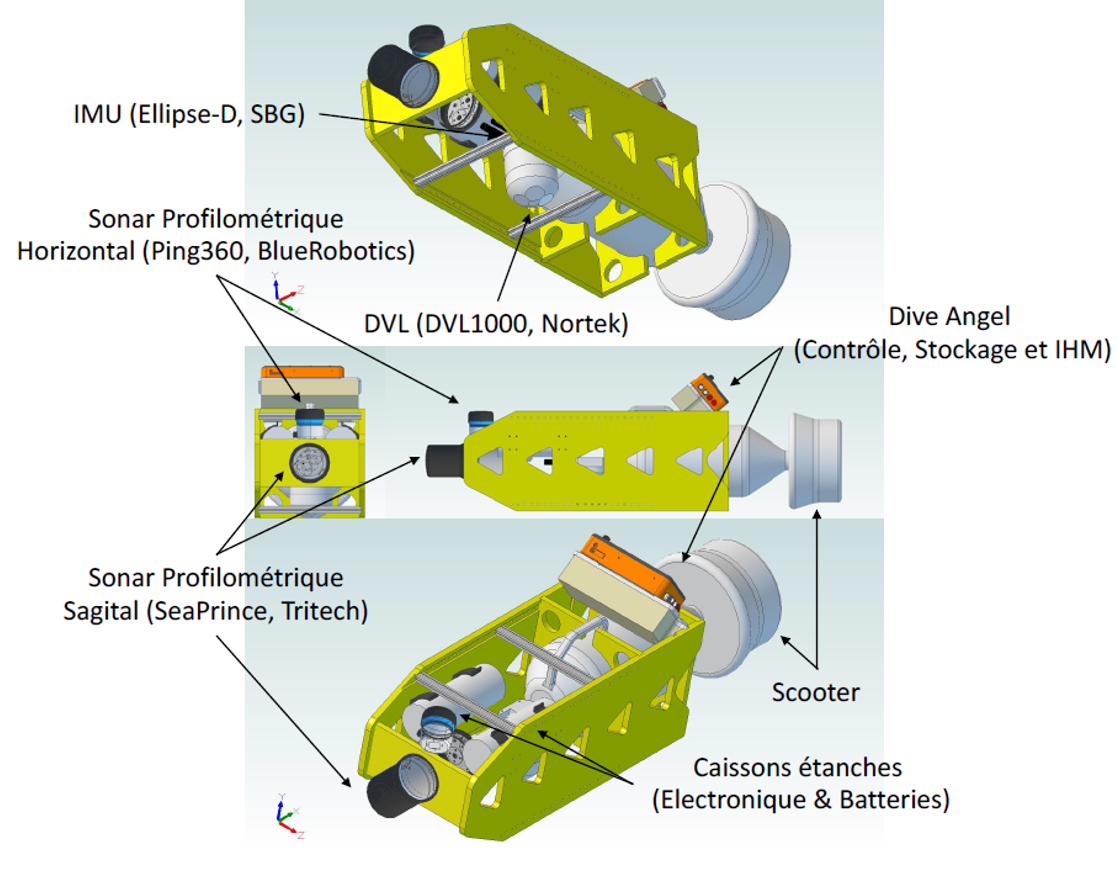
\includegraphics[width=\linewidth, height=5cm, keepaspectratio]{figures/Scooter.png}\\[0.3em]
    {\small (a)}
  \end{minipage}\hfill
  \begin{minipage}[b]{0.48\linewidth}    % right: the diver operating it
    \centering
    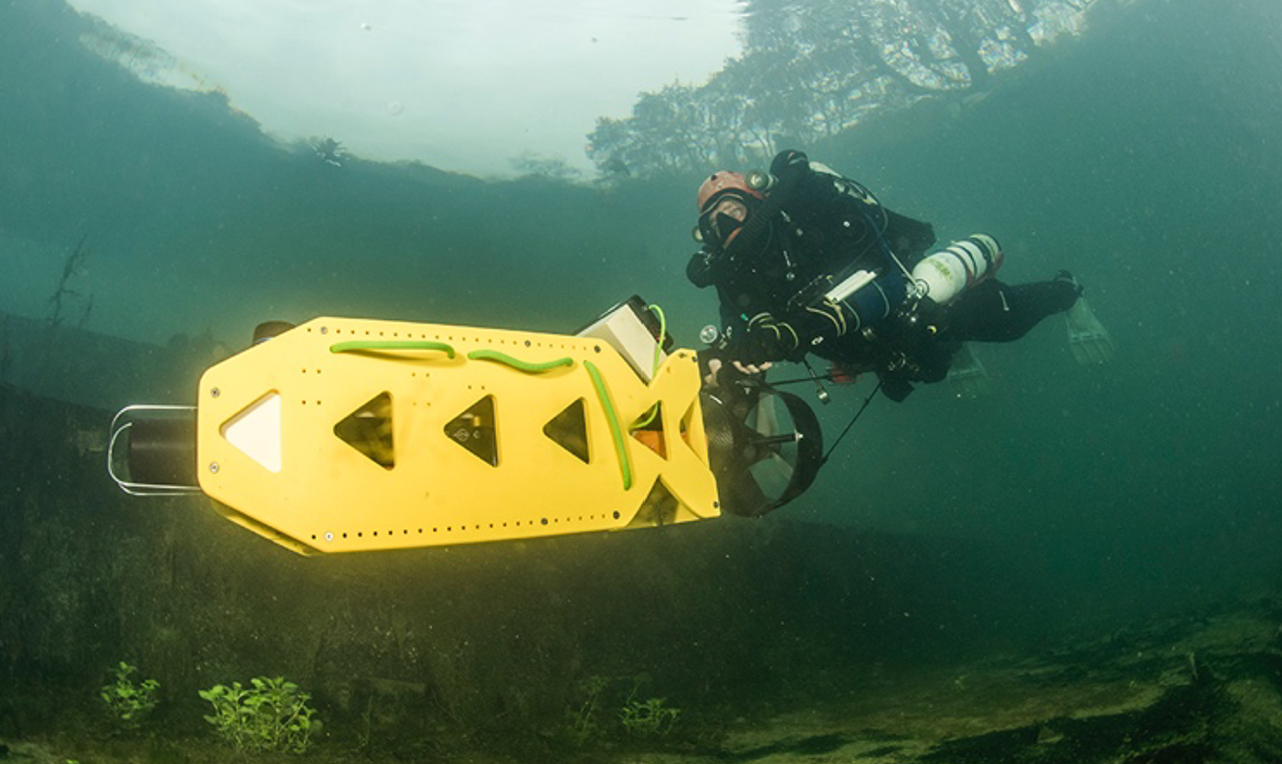
\includegraphics[width=\linewidth, height=5cm, keepaspectratio]{figures/Scooter_diver.png}\\[0.3em]
    {\small (b)}
  \end{minipage}
  \caption{The NavScoot~2 acquisition platform \citep{margaritis2025internship}: (a) the vehicle
           with its sensors; (b) the diver operating it.}
  \label{fig:bg_navscoot}
\end{figure}

% ------------------------------------------------------------------------------
\subsection{From raw data to a point cloud}  % the existing pipeline
\label{sec:bg_pipeline}                      % \secref{sec:bg_pipeline}

The previous work re-implemented the original MATLAB processing chain in Python and corrected
several errors in it \citep{margaritis2025internship}. The pipeline works in three stages:
\begin{enumerate}                        % pipeline stages in order
  \item \textbf{Trajectory.} DVL velocity spikes above 2~m/s are removed, all sensors are
        restricted to their common time window and expressed in the vehicle body frame. The
        velocity is rotated into the world frame with the IMU orientation and integrated over
        time, while the depth sensor gives the vertical position (dead reckoning).
  \item \textbf{Echo detection.} In every ping of the vertical sonar, the noise close to the
        transducer is cut, and the first return above an intensity threshold is kept as the
        distance to the conduit wall; later returns are discarded as multipath echoes.
  \item \textbf{Projection.} Each detection (range, beam angle, time) is placed in 3D using the
        vehicle pose interpolated at the time of the ping, giving a point cloud of about
        50\,000 points.
\end{enumerate}
Integrating velocities accumulates drift, which distorts the point cloud. It was reduced with the
Continuous-time SLAM of the 3D Toolkit (3DTK) \citep{borrmann2008globally, nuchter2017cartographer},
which splits the trajectory into overlapping segments and deforms it smoothly so that the parts
of the cloud that see the same walls align (Figure~\ref{fig:bg_pointcloud}). The corrected cloud
was then turned into a surface mesh with learning-based reconstruction methods.

\begin{figure}[!htbp]                    % the data this project starts from
  \centering
  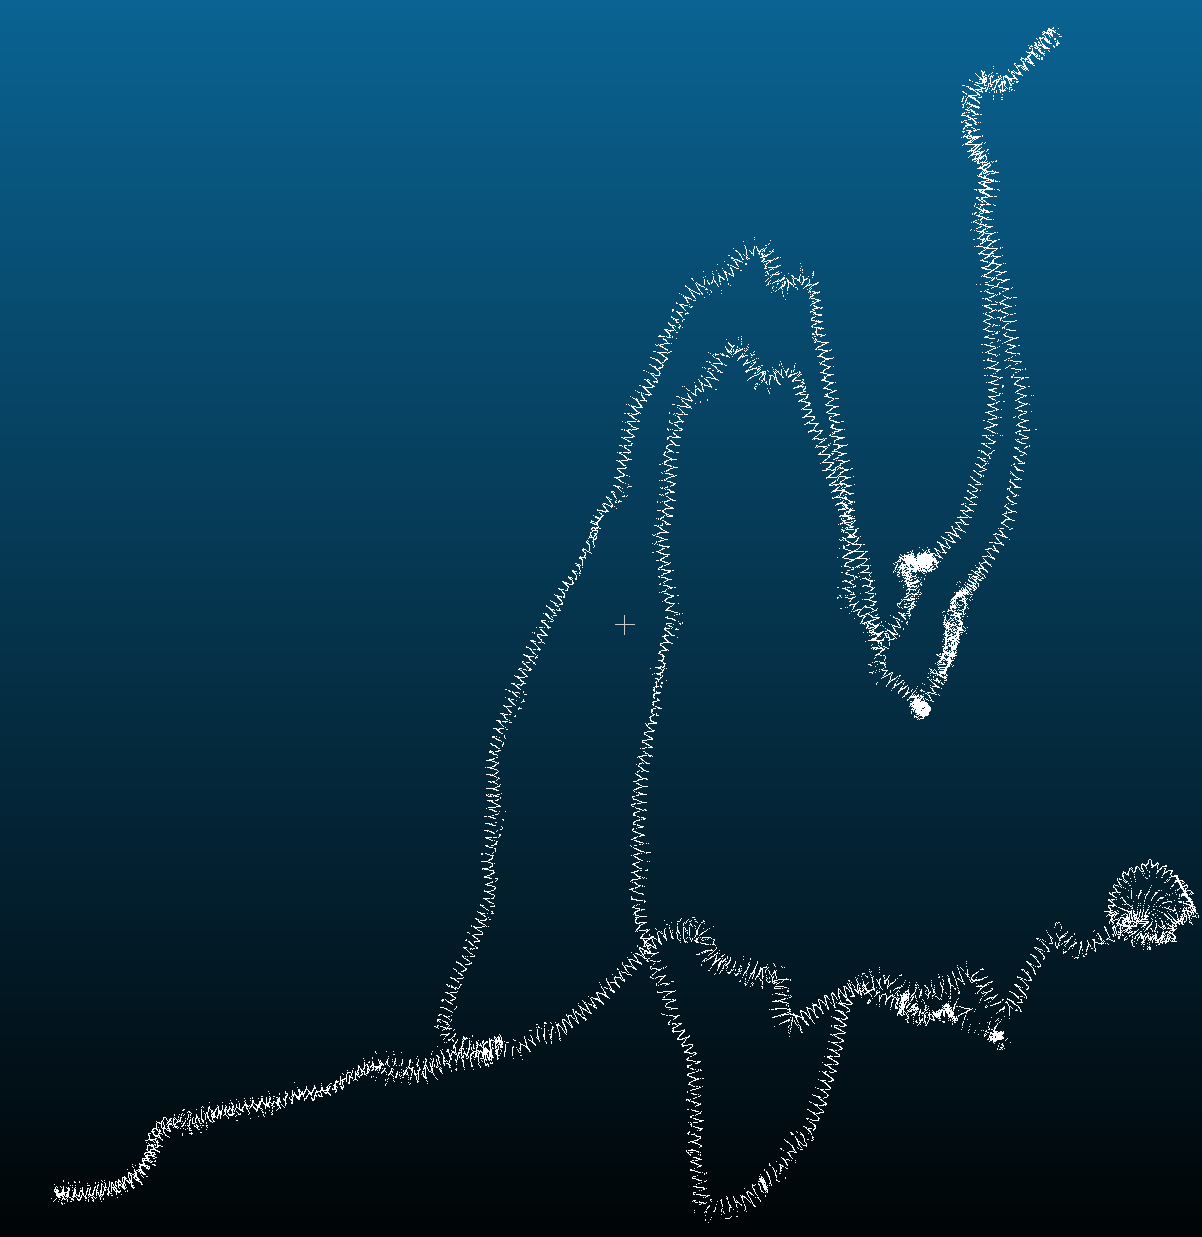
\includegraphics[width=0.9\linewidth, height=9cm, keepaspectratio]{figures/initial_point_cloud.png}
  \caption{Initial point cloud of the conduit obtained from the vertical sonar \citep{margaritis2025internship}.}
  \label{fig:bg_pointcloud}
\end{figure}

% ------------------------------------------------------------------------------
\subsection{The unused horizontal sonar}  % the gap this project addresses
\label{sec:bg_gap}                        % \secref{sec:bg_gap}

The point cloud of \citet{margaritis2025internship}, and everything built on it, uses only the
echoes of the vertical sonar. Each vertical scan describes one cross-section of the conduit, so
the map is a sequence of slices whose spacing along the conduit depends entirely on the estimated
trajectory. The horizontal sonar, recorded during the same dive, sees the walls along the
direction of travel and could provide extra information about the conduit geometry, but it was not used in that work.
(Figure~\ref{fig:bg_scanplanes}).

Exploiting it is, however, not trivial:
\begin{itemize}                          % why the horizontal sonar is hard to use
  \item \textbf{Elevation ambiguity:} with a beam 25$^\circ$ high, an echo may come from anywhere
        within that vertical aperture, so the height of a detected point is uncertain.
  \item \textbf{Motion during a scan:} a 360$^\circ$ sweep takes several seconds, during which the
        vehicle moves and turns, so each ping must be placed with its own pose.
  \item \textbf{Fusion of perpendicular scans:} the two sonars observe different planes, at
        different rates and with different noise, and must be expressed consistently in a single
        frame and point cloud.
\end{itemize}
The aim of this project is to process the horizontal sonar data and merge them with the vertical
sonar data into one consistent point cloud (\secref{sec:msis_merging}).

\begin{figure}[!htbp]                    % geometry of the two scanning planes
  \centering
  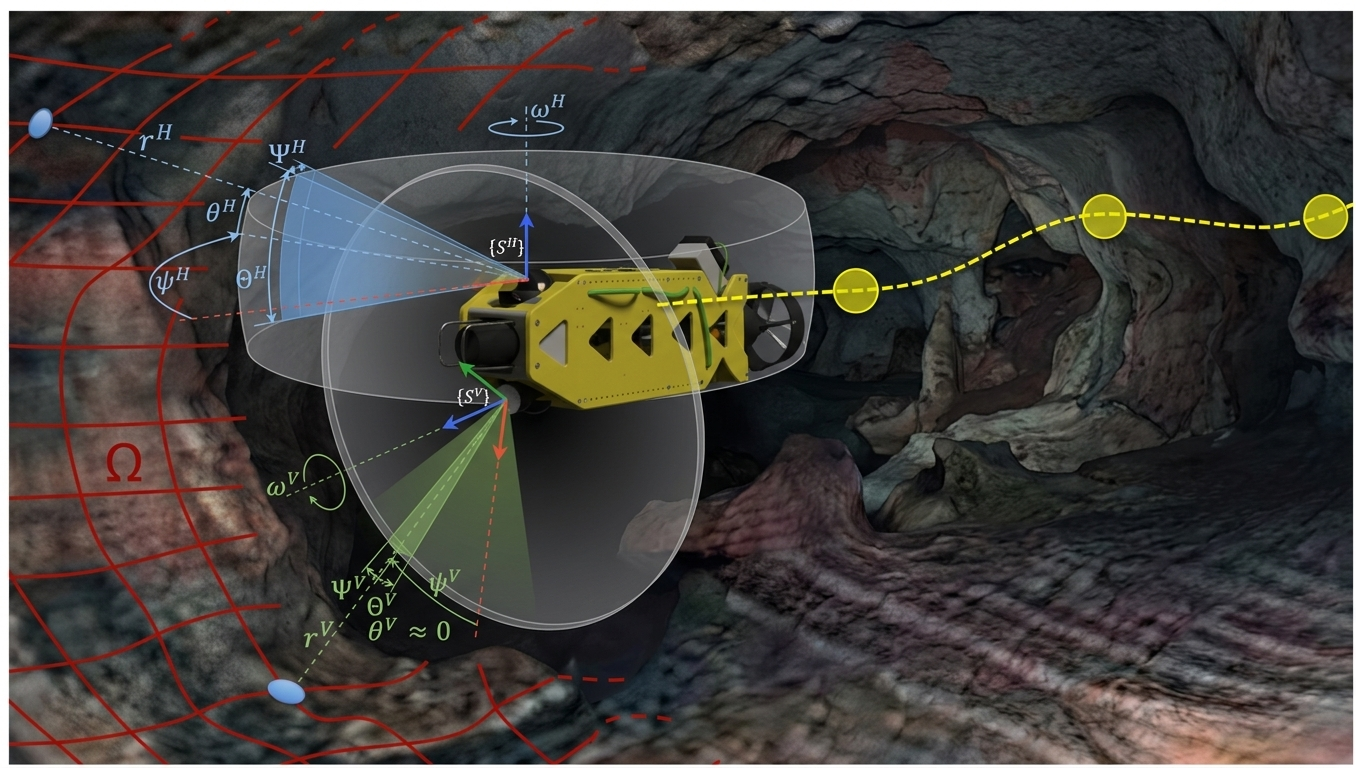
\includegraphics[width=0.9\linewidth, height=9cm, keepaspectratio]{figures/scanning_planes.jpeg}
  \caption{Scanning planes of the two MSIS on the NavScoot~2.}
  \label{fig:bg_scanplanes}
\end{figure}

\section{Introduction}                   % obligatory
\label{sec:introduction}                 % \secref{sec:introduction}

\hint{Briefly outline the company and/or department you worked for. Summarise the work
you have done and clearly state the objectives of your project. You can also state the
importance of your project and its relevance.}

\section{Definitions}                    % notation, frames and models used in the report
\label{sec:definitions}                  % \secref{sec:definitions}

The scan-merging method implemented in this project is the one proposed by
\citet{breux2020elevation} for a vehicle carrying the same pair of perpendicular sonars. This
section fixes the notation, frames and models of that work, adapted to the NavScoot~2, and
used in the rest of the report.

% ------------------------------------------------------------------------------
\subsection{Notation}                    % general conventions
\label{sec:def_notation}                 % \secref{sec:def_notation}

\begin{itemize}                          % one convention per item
  \item Vectors are written in bold lower case ($\mathbf{x}$) and matrices in upper case
        ($\mathbf{M}$). $\mathbf{x}|_{\{R\}}$ denotes a vector expressed in the frame $\{R\}$.
  \item $X \sim q(\lambda)$ means that the random variable $X$ follows the law of probability
        density function (pdf) $q$ with parameters $\lambda$; $\mathcal{N}(\boldsymbol{\mu},
        \boldsymbol{\Sigma})$ is the Gaussian law of mean $\boldsymbol{\mu}$ and covariance
        $\boldsymbol{\Sigma}$. $\hat{X}$ denotes an estimate of $X$.
  \item $SE(3)$ is the group of rigid transformations of space. A pose is stored as a position and a
        unit quaternion $\mathbf{q}$, whose rotation matrix is $\mathbf{R}(\mathbf{q})$, or as the
        equivalent $4\times4$ homogeneous matrix $\mathbf{T} = \begin{bmatrix} \mathbf{R} &
        \boldsymbol{\tau} \\ \mathbf{0} & 1 \end{bmatrix}$.
  \item $SE(3)$ is a Lie group; its Lie algebra $\mathfrak{se}(3)$ holds the infinitesimal motions,
        written as 6-vectors $\boldsymbol{\xi} = [\mathbf{v}^T\ \boldsymbol{\omega}^T]^T$ with a
        translational part $\mathbf{v}$ and a rotational part $\boldsymbol{\omega}$. The logarithm
        map $\log : SE(3) \to \mathfrak{se}(3)$ returns the motion that leads from the identity to a
        given transformation. $T_{\mathbf{A}}SE(3)$ is the tangent space of $SE(3)$ at
        $\mathbf{A}$ and $\langle \cdot, \cdot \rangle_{\mathbf{A}}$ an inner product on it; $e$ is
        the identity element.
  \item Orientations can also be given by Euler angles $[\psi\ \chi\ \phi]^T$ (yaw, pitch, roll),
        with rotation matrix $\mathbf{R}(\psi, \chi, \phi)$; these angles are written with a
        $\delta$ when they are increments, to distinguish them from the sonar angles $\psi^h$,
        $\psi^v$. $[\boldsymbol{\omega}]_\times$ is the skew-symmetric matrix such that
        $[\boldsymbol{\omega}]_\times \mathbf{x} = \boldsymbol{\omega} \times \mathbf{x}$.
  \item $\oplus$ (resp.\ $\ominus$) is the composition (resp.\ inverse composition) of poses and
        points \citep{blanco2010tutorial}: if $\boldsymbol{\eta}$ is the pose of a frame and
        $\mathbf{x}$ a point expressed in that frame, $\boldsymbol{\eta} \oplus \mathbf{x}$ is the same
        point expressed in the frame in which $\boldsymbol{\eta}$ is given. Conversely,
        $\mathbf{x} \ominus \boldsymbol{\eta}$ expresses in the frame of pose $\boldsymbol{\eta}$ a
        point $\mathbf{x}$ given in the reference frame.
\end{itemize}

% ------------------------------------------------------------------------------
\subsection{Frames and poses}            % where everything is expressed
\label{sec:def_frames}                   % \secref{sec:def_frames}

Four frames are used (Figure~\ref{fig:def_frames}a): the fixed world frame $\{0\}$, the body frame
$\{B\}$ attached to the vehicle, and the frames $\{S_H\}$ and $\{S_V\}$ attached to the horizontal
and vertical sonar heads. With these frames:
\begin{itemize}                          % pose vectors
  \item $\boldsymbol{\tau}$ ($3\times1$) and $\mathbf{q}$ ($4\times1$) are the position and attitude of
        $\{B\}$ in $\{0\}$, and $\boldsymbol{\eta} = [\boldsymbol{\tau}^T\ \mathbf{q}^T]^T$ ($7\times1$)
        is the \emph{pose} of the vehicle;
  \item $\mathbf{p}_H = [\boldsymbol{\tau}_H^T\ \mathbf{q}_H^T]^T$ and
        $\mathbf{p}_V = [\boldsymbol{\tau}_V^T\ \mathbf{q}_V^T]^T$ are the fixed poses of $\{S_H\}$ and
        $\{S_V\}$ in $\{B\}$, given by the mounting of the sonars on the NavScoot~2
        \citep{margaritis2025internship}.
\end{itemize}
The navigation sensors (DVL, IMU, depth sensor) provide by dead reckoning a pose estimate at regular
times, assumed Gaussian, $\boldsymbol{\eta} \sim \mathcal{N}(\bar{\boldsymbol{\eta}},
\boldsymbol{\Sigma}_{\eta})$. The \emph{discretized trajectory} is the set of these poses,
$\mathcal{H} = \{\boldsymbol{\eta}_i\}$, $i \in \{1,\dots,n_r\}$.

% ------------------------------------------------------------------------------
\subsection{Sonar measurements}          % what one ping gives
\label{sec:def_measurements}             % \secref{sec:def_measurements}

Both sonars are mechanically scanned imaging sonars (MSIS): a head rotates step by step around one
axis and, at each step, emits a ping whose echoes give the range $\rho$ to the surrounding surface
$\Omega$. In the sonar frame, a point is described by its range $\rho$, its \emph{rotation angle}
$\psi$ (the angle of the head) and its \emph{elevation angle} $\theta$, defined as the oriented angle
between the $XY$-plane of the sonar frame and the measured ray. A beam has a vertical aperture
$\Theta$ and a horizontal aperture $\Psi$. On the NavScoot~2, the vertical sonar beam
(1--2$^\circ$) and the horizontal width of the horizontal sonar beam (2$^\circ$) are narrow, so
we take $\Psi_H = \Psi_V = \Theta_V = 0$. Only the vertical aperture of the horizontal sonar
is kept: $\Theta_H = [-b/2,\, b/2]$, with $b = 25^\circ$ for the Ping360.

\begin{itemize}                          % the two kinds of measurement
  \item \textbf{Vertical sonar.} A ping gives a single point,
        $\mathbf{m}^v_k = [\rho^v_k\ \ 0\ \ \psi^v_k]^T$ in $\{S_V\}$: its elevation is known and
        equal to zero.
  \item \textbf{Horizontal sonar.} Because of the aperture $\Theta_H$, a single ping can return
        $n$ echoes at different ranges $\rho^h_{ij}$ and \emph{unknown} elevation angles
        $\theta^h_{ij}$, all with the same rotation angle $\psi^h_i$
        (Figure~\ref{fig:def_frames}b). The $i$-th measurement is the $3\times n$ matrix
        $\mathbf{M}^h_i = [\mathbf{m}^h_{ij}]$, with
        $\mathbf{m}^h_{ij} = [\rho^h_{ij}\ \ \theta^h_{ij}\ \ \psi^h_i]^T$.
\end{itemize}

A \emph{complete scan} $\mathcal{S} = \{\mathcal{M}^h, \mathcal{M}^v\}$ gathers the measurements
$\mathcal{M}^h = \{\mathbf{M}^h_i\}$, $i \in \{1,\dots,n_h\}$, taken while the horizontal sonar
completes a full $360^\circ$ rotation, and the measurements
$\mathcal{M}^v = \{\mathbf{m}^v_k\}$, $k \in \{1,\dots,n_v\}$, of the vertical sonar over the same
time interval. Since the sonars and the navigation are not synchronized, the functions
$\sigma^h : \{1,\dots,n_h\} \to \{1,\dots,n_r\}$ and $\sigma^v : \{1,\dots,n_v\} \to
\{1,\dots,n_r\}$ return the index of the pose at which each measurement was taken. A measurement
is then placed in the world frame by
\begin{equation}                         % spherical sonar coordinates -> world point
  g^h(\rho, \theta, \psi, i) = \boldsymbol{\eta}_{\sigma^h(i)} \oplus \mathbf{p}_H \oplus
  \begin{bmatrix} \rho\cos\theta\cos\psi \\ \rho\cos\theta\sin\psi \\ \rho\sin\theta \end{bmatrix},
  \label{eq:def_gh}
\end{equation}
and $g^v$ is defined in the same way with $\sigma^v$ and $\mathbf{p}_V$. For a vertical
measurement every argument is known. For a horizontal one, $\theta$ is missing: estimating it is
the goal of scan merging and in general the goal of this project.

\begin{figure}[!htbp]                    % frames and the elevation ambiguity
  \centering
  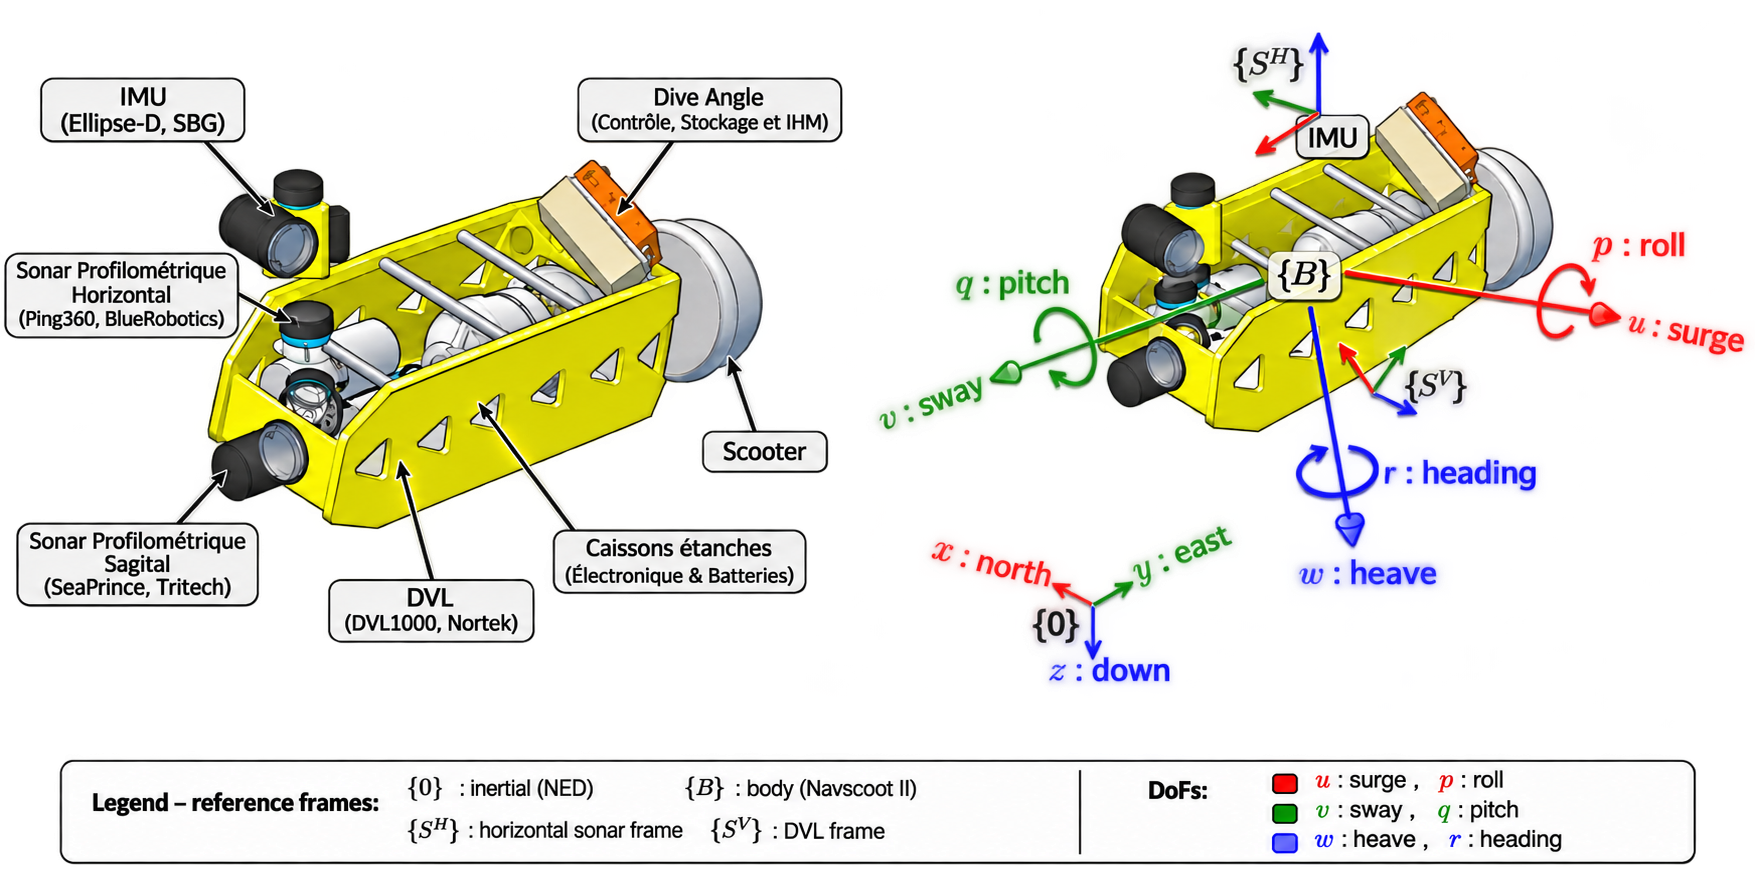
\includegraphics[width=0.8\linewidth, height=9cm, keepaspectratio]{figures/frames_used.png}\\[0.2em]
  {\small (a)}\\[0.8em]
  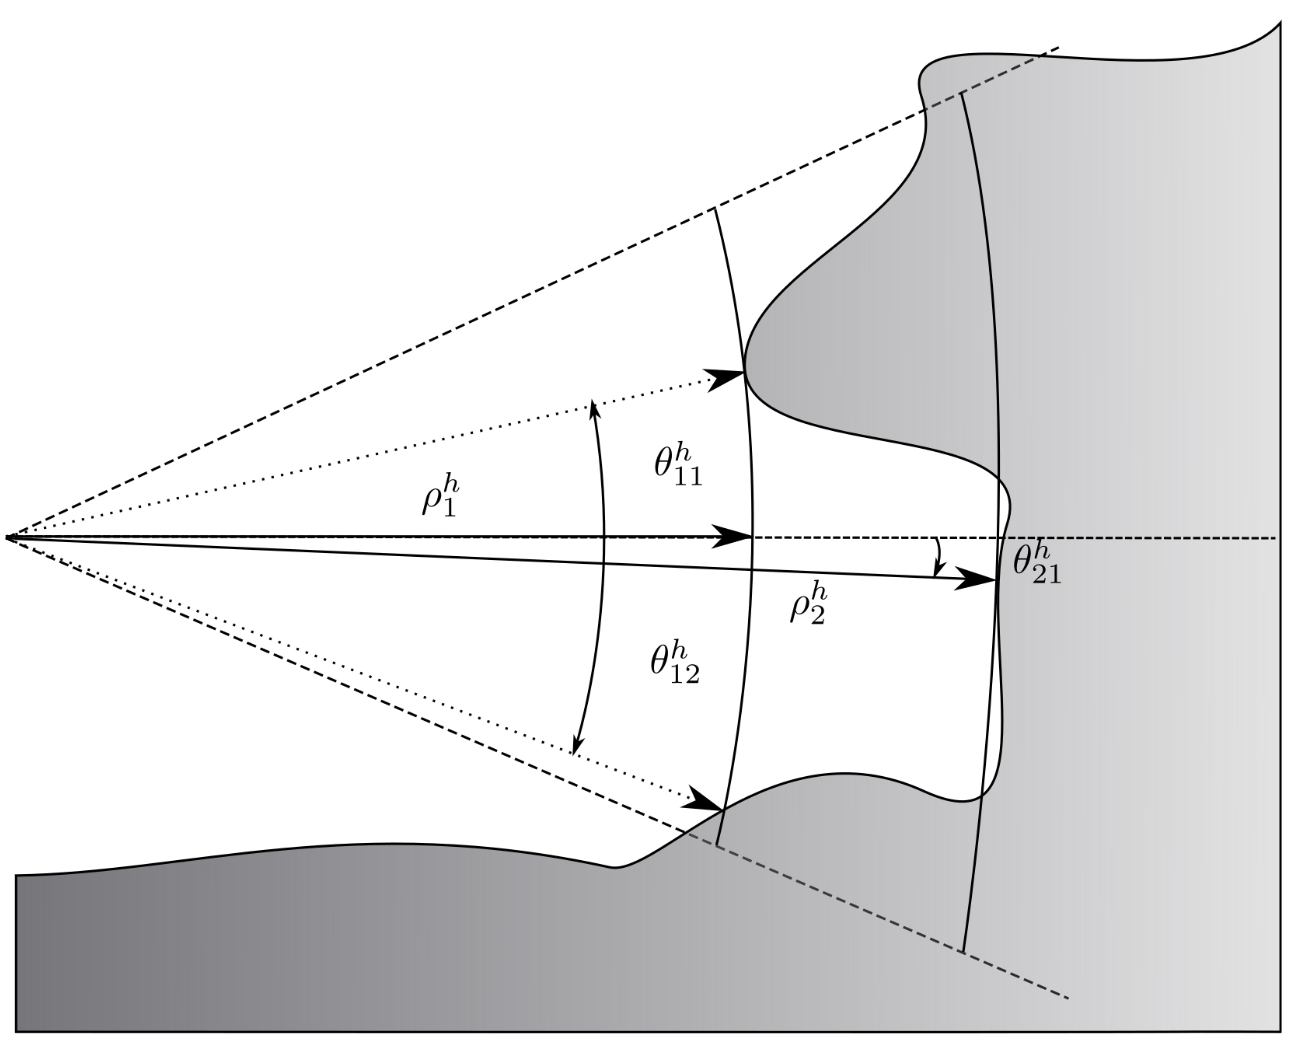
\includegraphics[width=0.8\linewidth, height=9cm, keepaspectratio]{figures/several_elevation_angles.png}\\[0.2em]
  {\small (b)}
  \caption{(a) Frames used in this report. (b) A single horizontal sonar ping can correspond to
           several 3D points, hence several elevation angles. Adapted from
           \citet{breux2020elevation}.}
  \label{fig:def_frames}
\end{figure}

% ------------------------------------------------------------------------------
\subsection{Gaussian process regression}  % the surface model
\label{sec:def_gp}                        % \secref{sec:def_gp}

A Gaussian process (GP) is a set of random variables of which every finite subset follows a joint
Gaussian law \citep{rasmussen2006gaussian}. A GP $f \sim \mathcal{GP}(f_p, K)$ is defined by a prior
mean function $f_p$ and a covariance function, or \emph{kernel}, $K(\mathbf{x}, \mathbf{x}')$, which
measures how similar the outputs at two inputs are expected to be. GP regression uses it as a
non-parametric model of an unknown function. Here it models the conduit surface seen by the
vertical sonar: the inputs are the curvilinear abscissa $s$ of the pose along the trajectory
(\secref{sec:msis_merging}) and the rotation angle $\psi^v$, and the output is the range,
\begin{equation}                         % observation model
  \rho^v = f(s, \psi^v) + e, \qquad e \sim \mathcal{N}(0, \sigma_n^2).
  \label{eq:def_gp_model}
\end{equation}
Given $N$ training inputs $\mathbf{X}$ with observed ranges $\mathbf{y}$, the prediction at a new input
$\mathbf{x}_*$ is Gaussian, $\rho_* \sim \mathcal{N}(\bar{\rho}_*, \sigma^2_{\rho_*})$, with
\begin{align}                            % GP posterior mean and variance
  \bar{\rho}_*      &= f_p(\mathbf{x}_*) + \mathbf{k}_*^T(\mathbf{K} + \sigma_n^2\mathbf{I})^{-1}
                       \big(\mathbf{y} - f_p(\mathbf{X})\big), \label{eq:def_gp_mean}\\
  \sigma^2_{\rho_*} &= K(\mathbf{x}_*, \mathbf{x}_*) - \mathbf{k}_*^T(\mathbf{K} +
                       \sigma_n^2\mathbf{I})^{-1}\mathbf{k}_*, \label{eq:def_gp_var}
\end{align}
where $\mathbf{K}$ is the $N\times N$ matrix of kernel values between training inputs and
$\mathbf{k}_*$ the vector of kernel values between $\mathbf{x}_*$ and the training inputs. The
variance gives the confidence band around the estimated surface.

The kernel sets the smoothness of the estimated surface. The default choice is the radial basis
function (RBF) kernel; the Mat\'ern family \citep{matern1986spatial} generalizes it with a parameter
$\nu$ that controls smoothness, from the rough exponential kernel ($\nu = 1/2$) to the RBF kernel
($\nu \to \infty$), with $\nu = 3/2$ as a compromise:
\begin{equation}                         % kernels used later
  K_{\mathrm{RBF}}(\mathbf{x}, \mathbf{x}') = \sigma_p^2\, e^{-\frac{r^2}{2l^2}}, \qquad
  K_{\mathrm{exp}}(\mathbf{x}, \mathbf{x}') = \sigma_p^2\, e^{-\frac{r}{l}}, \qquad
  K^M_{3/2}(\mathbf{x}, \mathbf{x}') = \sigma_p^2 \Big(1 + \tfrac{\sqrt{3}\,r}{l}\Big)
                                       e^{-\frac{\sqrt{3}\,r}{l}},
  \label{eq:def_kernels}
\end{equation}
with $r = \|\mathbf{x} - \mathbf{x}'\|$, $\sigma_p^2$ the signal variance and $l$ the length scale.
The hyperparameters $l$, $\sigma_p$ and $\sigma_n$ are set by hand or by maximum likelihood on the
training data. Products and sums of kernels are also kernels, which allows a kernel to be built for
a given problem.

% ------------------------------------------------------------------------------
\subsection{Scaled beta distribution}    % uncertainty of an elevation angle
\label{sec:def_beta}                     % \secref{sec:def_beta}

An estimated elevation angle $\hat{\theta}$ can only lie inside the beam, so its uncertainty is not
modelled by a Gaussian, whose support is infinite, but by a beta distribution scaled to
$[-b/2,\, b/2]$ \citep{johnson1994continuous, breux2020elevation}:
\begin{equation}                         % scaled beta pdf
  p(\theta;\, \alpha, \beta, b) = \frac{\Gamma(\alpha+\beta)}{\Gamma(\alpha)\,\Gamma(\beta)}\,
  \frac{(\theta + \frac{b}{2})^{\alpha-1}\,(\frac{b}{2} - \theta)^{\beta-1}}{b^{\alpha+\beta-1}},
  \qquad \theta \in \Big[-\frac{b}{2}, \frac{b}{2}\Big],
  \label{eq:def_beta}
\end{equation}
where $\Gamma$ is the gamma function, which extends the factorial to real and complex numbers,
\begin{equation}                         % gamma function
  \Gamma(z) = \int_0^{\infty} x^{z-1} e^{-x}\, dx, \qquad \operatorname{Re}(z) > 0.
  \label{eq:def_gamma}
\end{equation}
The shape parameters follow from a mean $\bar{\theta}$ and a variance $\sigma_\theta^2$:
\begin{equation}                         % moment matching
  \alpha = (b + 2\bar{\theta})\,\frac{b^2 - 4(\bar{\theta}^2 + \sigma_\theta^2)}{8b\,\sigma_\theta^2},
  \qquad
  \beta  = (b - 2\bar{\theta})\,\frac{b^2 - 4(\bar{\theta}^2 + \sigma_\theta^2)}{8b\,\sigma_\theta^2}.
  \label{eq:def_beta_params}
\end{equation}
For $\alpha = \beta = 1$ it reduces to the uniform distribution on the beam, $p = 1/b$, which is the
only information available on $\theta$ without scan merging.

% ------------------------------------------------------------------------------
% \subsection{Acronyms}                    % abbreviations used in the report
% \label{sec:def_acronyms}                 % \secref{sec:def_acronyms}

% \begin{table}[!htbp]                     % two (acronym, meaning) column pairs side by side
%   \centering
%   \small
%   \begin{tabular}{ll@{\hspace{2em}}ll}
%     \toprule
%     DVL  & Doppler velocity log                 & MSIS & Mechanically scanned imaging sonar \\
%     GP   & Gaussian process                     & pdf  & Probability density function       \\
%     IMU  & Inertial measurement unit            & RBF  & Radial basis function              \\
%     MLE  & Maximum likelihood estimation        & SLAM & Simultaneous localization and mapping \\
%     \bottomrule
%   \end{tabular}
%   \caption{Acronyms used in this report.}
%   \label{tab:def_acronyms}
% \end{table}

\section{MSIS Scan Merging}              % the method implemented in this project
\label{sec:msis_merging}                 % \secref{sec:msis_merging}

The horizontal sonar of the NavScoot~2 measures the range of every echo but not its elevation
inside its $25^\circ$ beam (\secref{sec:def_measurements}). A wide beam is nevertheless valuable:
it covers a large part of the conduit at each rotation, which increases the surface seen by two
successive $360^\circ$ scans and therefore the chance of recognizing a region already mapped. The
price is a high uncertainty on the 3D position of each echo \citep{breux2020elevation}. This
project implements the method of \citet{breux2020elevation} to reduce this uncertainty. Its key
idea is that both sonars observe the same environment, which is the variable linking their
measurements. The measurements of the high-resolution, narrow-beam vertical sonar are used to build
a probabilistic approximation of the surrounding surface by Gaussian process regression; this
surface is then used to estimate the probability distribution of the elevation angles of the
low-resolution, wide-beam horizontal sonar. In \citet{margaritis2025internship}, the vertical sonar
was only used to add points to the reconstructed environment; here it is also used to estimate the
elevation angles of the horizontal sonar.

The method only considers the trajectory during the acquisition of one complete scan
(\secref{sec:def_measurements}): the measurements $\mathcal{M}^h$ of one full rotation of the
horizontal sonar, the measurements $\mathcal{M}^v$ of the vertical sonar during the same interval,
and the dead-reckoning poses $\mathcal{H} = \{\boldsymbol{\eta}_i\}$, $i \in \{1,\dots,n_r\}$, of
that interval. The estimation of the full trajectory, for instance in a pose-graph SLAM framework,
is outside the scope of the method.

% ==============================================================================
\subsection{Environment model}           % how the conduit wall is parameterized
\label{sec:msis_model}                   % \secref{sec:msis_model}

The surface of the environment is modelled through \emph{virtual vertical sonar measurements}: a 3D
point on the surface is parameterized by the 6D pose of the vehicle and the rotation angle of the
vertical sonar at which this point could have been seen by the vertical sonar. Formally, the surface
is defined as the function
\begin{equation}                         % surface as a function of pose and sonar angle
  f : \left\{
  \begin{array}{rcl}
    SE(3) \times [-\pi, \pi] & \to     & \mathbb{R}^+ \\
    (\boldsymbol{\eta}, \psi^v) & \mapsto & \rho^v
  \end{array}\right.
  \label{eq:msis_surface}
\end{equation}
which maps a pose $\boldsymbol{\eta}$ and a rotation angle $\psi^v$ to the distance $\rho^v$,
expressed in the scanning plane of the vertical sonar (the $XY$-plane of $\{S_V\}$), that would have
been measured from the pose $\boldsymbol{\eta}$ with the rotation angle $\psi^v$. A terrain model of
the form $z = f(x, y)$, common in seafloor mapping, cannot be used here: in a conduit, $z$ is not a
function of $(x, y)$, since a vertical line crosses the wall both at the floor and at the roof.

The trajectory of the vehicle is a one-dimensional submanifold of $SE(3)$, so it can be
parameterized by a single scalar $u \in \mathbb{R}$. Since a kernel measures the similarity of two
inputs (\secref{sec:def_gp}), this parameter must be such that, for a kernel $K$,
\begin{equation}                         % requirement on the trajectory parameter
  K(\boldsymbol{\eta}_1, \boldsymbol{\eta}_2) = K(u_1, u_2).
  \label{eq:msis_kernelreq}
\end{equation}
The time $t$ does not satisfy Eq.~\eqref{eq:msis_kernelreq}: the length scale $l$ of the kernel
(Eq.~\eqref{eq:def_kernels}) would depend on time and not on space. For instance, a vehicle standing
still at two instants $t_2 \gg t_1$ has $\boldsymbol{\eta}(t_1) = \boldsymbol{\eta}(t_2)$, so that
$K(\boldsymbol{\eta}_1, \boldsymbol{\eta}_2) = \sigma_p^2$, whereas $K(t_1, t_2) \approx 0$.

The trajectory is instead parameterized by its \emph{curvilinear abscissa}, i.e.\ its length in
$SE(3)$. Lengths are measured with the left-invariant Riemannian metric used by
\citet{breux2020elevation}: for $\mathbf{A} \in SE(3)$ and two tangent vectors
$\mathbf{U}_1, \mathbf{U}_2 \in T_{\mathbf{A}}SE(3)$,
\begin{equation}                         % left-invariant metric on SE(3)
  \langle \mathbf{U}_1, \mathbf{U}_2 \rangle_{\mathbf{A}}
  = \langle \mathbf{A}^{-1}\mathbf{U}_1, \mathbf{A}^{-1}\mathbf{U}_2 \rangle_e
  = \operatorname{Tr}(\mathbf{S}_1^T \mathbf{S}_2)
  = \boldsymbol{\xi}_1^T \mathbf{G}\, \boldsymbol{\xi}_2, \qquad
  \mathbf{G} = \begin{bmatrix} \mathbf{I}_3 & \mathbf{0} \\ \mathbf{0} & 2\mathbf{I}_3 \end{bmatrix},
  \label{eq:msis_metric}
\end{equation}
where $\mathbf{S}_j = \mathbf{A}^{-1}\mathbf{U}_j \in \mathfrak{se}(3)$ and $\boldsymbol{\xi}_j$ is
the same element written as a 6-vector $[\mathbf{v}^T\ \boldsymbol{\omega}^T]^T$. The factor $2$ on
the rotational part comes from the trace:
$\operatorname{Tr}([\boldsymbol{\omega}]_\times^T[\boldsymbol{\omega}]_\times) = 2\lVert\boldsymbol{\omega}\rVert^2$.
The length of a curve $\boldsymbol{\eta}(t)$ in $SE(3)$ between two instants $t_1$ and $t_2$ is then
\begin{equation}                         % length of a curve in SE(3)
  L_{\boldsymbol{\eta}(t_1)}^{\boldsymbol{\eta}(t_2)} = \int_{t_1}^{t_2}
  \left\langle \frac{d\boldsymbol{\eta}}{dt}, \frac{d\boldsymbol{\eta}}{dt} \right\rangle_{\boldsymbol{\eta}(t)}^{1/2} dt,
  \label{eq:msis_length}
\end{equation}
and the curvilinear abscissa is the length travelled since the start of the scan,
\begin{equation}                         % continuous curvilinear abscissa
  s(t) = L_{\boldsymbol{\eta}(0)}^{\boldsymbol{\eta}(t)}.
  \label{eq:msis_abscissa_cont}
\end{equation}
The trajectory available here is the discrete set $\mathcal{H}$ of poses estimated by dead reckoning
from the DVL, the IMU and the depth sensor, so the length is approximated by summing the lengths of
the relative motions between consecutive poses. With $\mathbf{T}_k$ the $4\times4$ matrix of the pose
$\boldsymbol{\eta}_k$, $s_1 = 0$ and, for $i \in \{2,\dots,n_r\}$,
\begin{equation}                         % discrete curvilinear abscissa
  \begin{aligned}
    s_i = L_{\boldsymbol{\eta}_1}^{\boldsymbol{\eta}_i}
    &\approx \sum_{k=2}^{i} \langle \Delta\boldsymbol{\eta}_k, \Delta\boldsymbol{\eta}_k \rangle^{1/2}
     = \sum_{k=2}^{i} \sqrt{\log(\mathbf{T}_{k-1}^{-1}\mathbf{T}_k)^T\, \mathbf{G}\,
       \log(\mathbf{T}_{k-1}^{-1}\mathbf{T}_k)}
     = \sum_{k=2}^{i} \big\lVert \log(\mathbf{T}_{k-1}^{-1}\mathbf{T}_k) \big\rVert_G,
  \end{aligned}
  \label{eq:msis_abscissa}
\end{equation}
where $\mathbf{T}_{k-1}^{-1}\mathbf{T}_k$ is the motion from $\boldsymbol{\eta}_{k-1}$ to
$\boldsymbol{\eta}_k$ (written $\boldsymbol{\eta}_k \ominus \boldsymbol{\eta}_{k-1}$ by
\citealt{breux2020elevation}), $\log$ the logarithm map of $SE(3)$ and
$\lVert\boldsymbol{\xi}\rVert_G = \sqrt{\boldsymbol{\xi}^T\mathbf{G}\,\boldsymbol{\xi}}$. The abscissa
therefore grows with both the distance travelled and the rotation of the vehicle: a pure rotation
of 1~rad adds $\sqrt{2}$ to $s$, as much as a translation of $\sqrt{2}$~m.

The objective is then to estimate $f$ by training a Gaussian process on the vertical sonar
measurements, as a function $f(s, \psi^v)$ of the curvilinear abscissa and the rotation angle. The
learned function is finally used to estimate the most likely elevation angles $\theta^h_{ij}$ inside
the beams of the horizontal sonar.

% ==============================================================================
\subsection{Algorithm description}       % Algorithm 1 and its stages
\label{sec:msis_algorithm}               % \secref{sec:msis_algorithm}

The algorithm is summarized in Algorithm~\ref{alg:msis_merging} (\secref{sec:msis_pseudocode}). First, the curvilinear abscissa of
every pose of the trajectory is computed with Eq.~\eqref{eq:msis_abscissa} (lines 1--5). The
vertical sonar measurements are then placed in the world frame and an elliptic cylinder is fitted to
them as the surface prior $f_p$ (lines 6--7, \secref{sec:msis_prior}). The Gaussian process
modelling the surface is trained on the vertical sonar measurements and their curvilinear abscissae
(lines 8--10, \secref{sec:msis_gp}). Then, for every echo of every horizontal measurement, the most
likely elevation angles are estimated (line 14, Algorithm~\ref{alg:msis_mle},
\secref{sec:msis_mle}) and their uncertainties are computed (line 16,
Algorithm~\ref{alg:msis_uncertainty}, \secref{sec:msis_uncertainty}). Finally, each estimated angle
turns the echo into a 3D point with a known uncertainty, which is added to the vertical sonar points
of the scan (line 17). This last step is specific to this project, whose aim is a single point cloud
combining both sonars; \citet{breux2020elevation} stop at the distributions $p(\hat{\theta})$.

% ------------------------------------------------------------------------------
\subsubsection{Environment prior}        % elliptic cylinder fitted to the vertical points
\label{sec:msis_prior}                   % \secref{sec:msis_prior}

The prior $f_p$ is the mean function of the Gaussian process: it encodes what is known of the shape
of the environment before the regression, so that the process only has to learn how the real
surface deviates from it. Based on the typical geometry of karst conduits, the natural choice is an
\emph{elliptic cylinder}. For a pose $\boldsymbol{\eta} = [\boldsymbol{\tau}^T\ \mathbf{q}^T]^T$ on
the trajectory (equivalently, its curvilinear abscissa) and a rotation angle $\psi^v$,
$f_p(\boldsymbol{\eta}, \psi^v)$ returns the distance to the prior shape along the corresponding ray
of the vertical sonar. Let the cylinder have the pose $\mathbf{T}_c = [\mathbf{R}_c\ \boldsymbol{\tau}_c]$,
with its axis along the $z$-axis of its frame and the semi-axes $r_1$ and $r_2$ of its elliptic
section along the $x$- and $y$-axes. The ray starts at the sonar head
$\mathbf{o} = \boldsymbol{\tau} + \mathbf{R}(\mathbf{q})\boldsymbol{\tau}_V$ with the unit direction
$\mathbf{u} = \mathbf{R}(\mathbf{q})\mathbf{R}(\mathbf{q}_V)[\cos\psi^v\ \ \sin\psi^v\ \ 0]^T$.
Expressed in the frame of the cylinder, $\mathbf{o}' = \mathbf{R}_c^T(\mathbf{o} - \boldsymbol{\tau}_c)$
and $\mathbf{u}' = \mathbf{R}_c^T\mathbf{u}$, and $f_p(\boldsymbol{\eta}, \psi^v)$ is the smallest
positive root $\lambda$ of the polynomial equation of degree two
\begin{equation}                         % ray-cylinder intersection
  \left(\frac{o'_x + \lambda u'_x}{r_1}\right)^2 + \left(\frac{o'_y + \lambda u'_y}{r_2}\right)^2 = 1.
  \label{eq:msis_prior}
\end{equation}

Fitting this primitive to the vertical sonar points
$\mathcal{P}^v = \{\mathbf{p}_k = g^v(\rho^v_k, 0, \psi^v_k, k)\}$ is a non-linear optimization,
which, like any such optimization, needs a good initial shape. It is done in three steps
\citep{breux2020elevation}:
\begin{enumerate}                        % fitting steps
  \item \textbf{Initial axes.} A robust principal component analysis (RPCA) of $\mathcal{P}^v$ gives
        its centre $\mathbf{c}$ and three principal vectors $\mathbf{a}_1$, $\mathbf{a}_2$,
        $\mathbf{a}_3$. For a perfect elliptic cylinder, they correspond to the cylinder axis and the
        major and minor axes of the ellipse. If the cylinder were longer than wide, its axis would be
        the principal vector with the largest eigenvalue, but this cannot be assumed here, since one
        scan covers a short portion of conduit. The axis is instead found from tangent vectors:
        successive points of the vertical sonar lie on the same cross-section of the conduit, so the
        vector $\mathbf{t}_k = \mathbf{p}_{k+1} - \mathbf{p}_k$ approximates a tangent to the wall that
        is orthogonal to the axis, and its projection on the axis is minimal:
        \begin{equation}                 % choice of the cylinder axis
          \mathbf{a}_{\mathrm{axis}} = \arg\min_{\mathbf{a} \in \{\mathbf{a}_1, \mathbf{a}_2, \mathbf{a}_3\}}
          \sum_{k} \langle \mathbf{a}, \mathbf{t}_k \rangle^2.
          \label{eq:msis_axis_pca}
        \end{equation}
  \item \textbf{Elliptic section.} The points are projected on the plane spanned by the two other
        principal vectors, and an ellipse is fitted to these 2D projections. The PCA basis is then
        rotated around the cylinder axis to align it with the axes of the ellipse, which gives the
        initial pose $\mathbf{T}_c$ and semi-axes $r_1$, $r_2$.
  \item \textbf{Refinement.} The asymmetric distribution of the vertical sonar points has a large
        influence on the RPCA result (Figure~\ref{fig:msis_prior}). The cylinder is therefore refined
        with the Levenberg--Marquardt (LM) algorithm, which finds the shape minimizing the orthogonal
        distances $d_\perp$ of the points to the cylinder:
        \begin{equation}                 % orthogonal least squares
          \hat{\mathbf{x}} = \arg\min_{\mathbf{x} \in \mathbb{R}^8}\ \sum_{k=1}^{n_v} d_\perp(\mathbf{p}_k, \mathbf{x})^2,
          \label{eq:msis_lm}
        \end{equation}
        where $\mathbf{x}$ gathers the 6D pose $\mathbf{T}_c \in SE(3)$ of the cylinder and its two
        semi-axes. The pose is optimized on the manifold $SE(3)$ \citep{blanco2010tutorial}: each LM
        step computes an increment in $\mathfrak{se}(3)$, which is mapped back onto $SE(3)$ by the
        exponential map.
\end{enumerate}

\begin{figure}[!htb]                     % elliptic cylinder prior
  \centering
  \begin{minipage}[b]{0.32\linewidth}    % (a) vertical sonar points
    \centering
    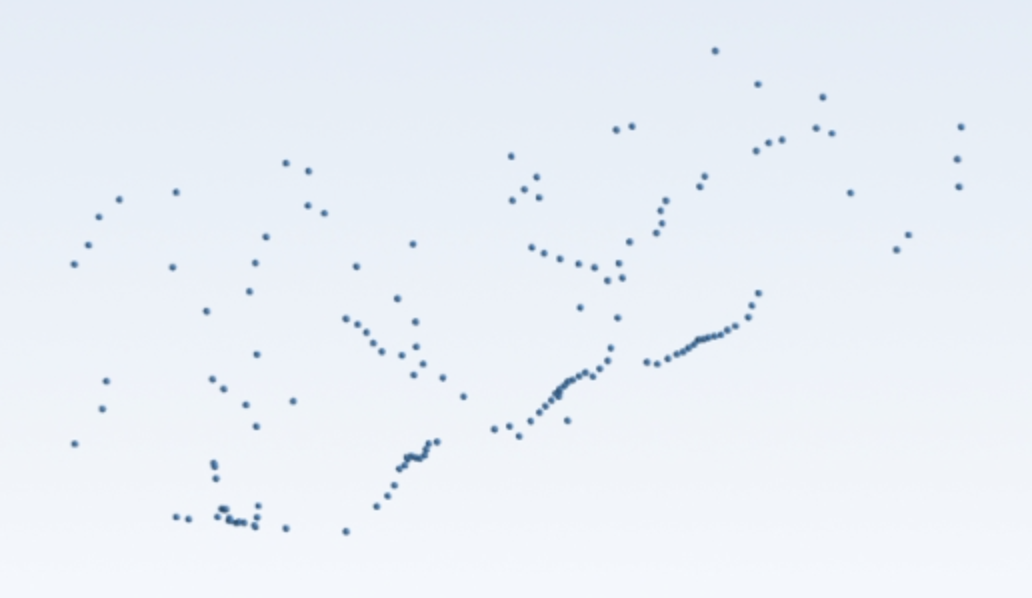
\includegraphics[width=\linewidth, height=4.5cm, keepaspectratio]{figures/points.png}\\[0.2em]
    {\small (a)}
  \end{minipage}\hfill
  \begin{minipage}[b]{0.32\linewidth}    % (b) initial cylinder from the RPCA
    \centering
    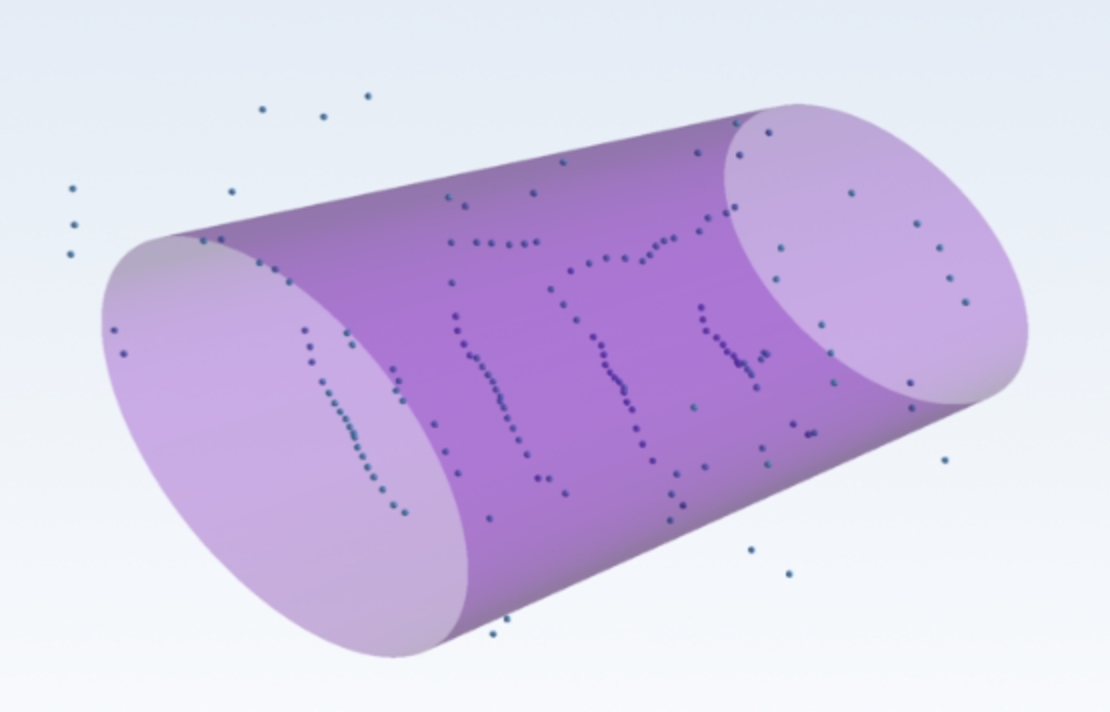
\includegraphics[width=\linewidth, height=4.5cm, keepaspectratio]{figures/initial_cyliner.png}\\[0.2em]
    {\small (b)}
  \end{minipage}\hfill
  \begin{minipage}[b]{0.32\linewidth}    % (c) cylinder after LM optimization
    \centering
    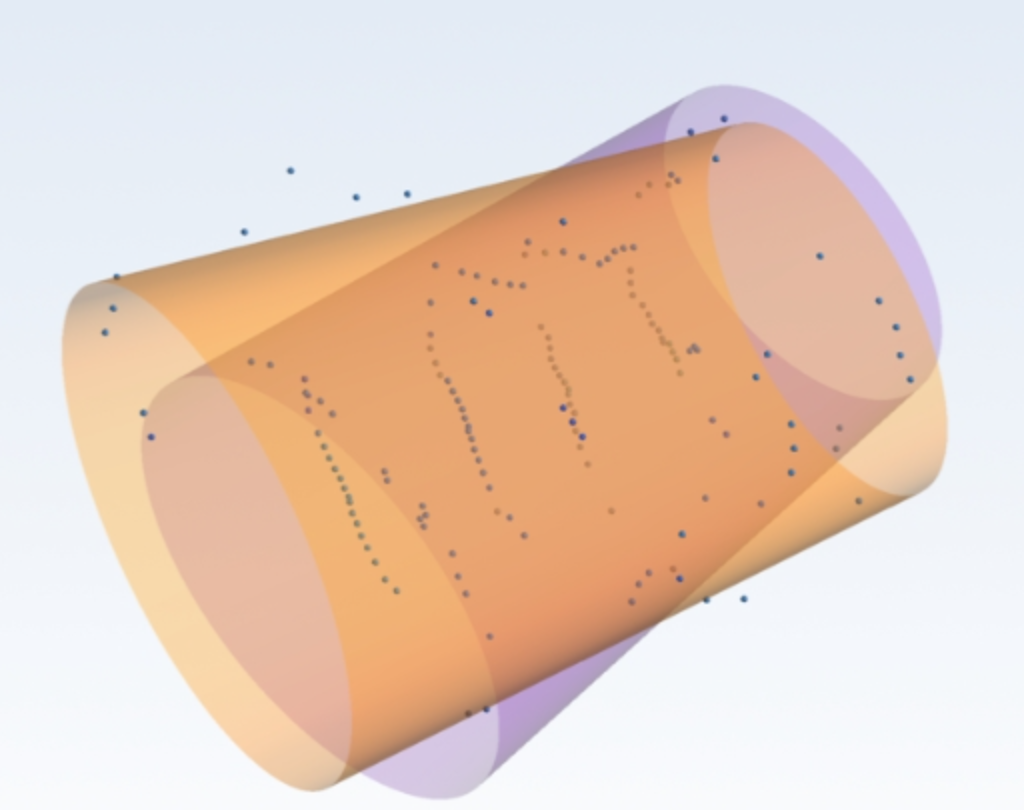
\includegraphics[width=\linewidth, height=4.5cm, keepaspectratio]{figures/optimised.png}\\[0.2em]
    {\small (c)}
  \end{minipage}
  \caption{Elliptic cylinder prior fitted to the vertical sonar points of one scan: (a) the vertical
           sonar points, (b) the initial cylinder estimated by RPCA, (c) the final cylinder after
           Levenberg--Marquardt optimization.}
  \label{fig:msis_prior}
\end{figure}

% ------------------------------------------------------------------------------
\subsubsection{Gaussian process regression and kernel choices}  % training the surface model
\label{sec:msis_gp}                                              % \secref{sec:msis_gp}

Each vertical measurement $\mathbf{m}^v_k$ provides one training input, the abscissa of its pose and
its rotation angle $\mathbf{x}_k = [s_{\sigma^v(k)}\ \ \psi^v_k]^T$, and one output, its range
$\rho^v_k$. They form the training set $\mathbf{X} = [\mathbf{x}_1 \dots \mathbf{x}_{n_v}]$,
$\mathbf{y} = [\rho^v_1 \dots \rho^v_{n_v}]^T$ of the Gaussian process
$f \sim \mathcal{GP}(f_p, K)$ of Eq.~\eqref{eq:def_gp_model}. The kernel exploits the cylindrical
structure of the surface by combining a kernel on the trajectory abscissa and a kernel on the
rotation angle:
\begin{equation}                         % product kernel
  K_{\mathrm{prod}}\big([s\ \psi^v]^T, [s'\ \psi'^v]^T\big) = K_s(s, s')\, K_\psi(\psi^v, \psi'^v).
  \label{eq:msis_kernel}
\end{equation}
$K_s$ can be any kernel of \secref{sec:def_gp}, or the Mat\'ern 5/2 kernel
\citep{rasmussen2006gaussian}
\begin{equation}                         % Matern 5/2 kernel
  K^M_{5/2}(\mathbf{x}, \mathbf{x}') = \sigma_p^2 \left(1 + \frac{\sqrt{5}\,r}{l} + \frac{5r^2}{3l^2}\right)
  e^{-\frac{\sqrt{5}\,r}{l}}, \qquad r = \lVert \mathbf{x} - \mathbf{x}' \rVert.
  \label{eq:msis_matern52}
\end{equation}
For $K_\psi$, a simple Euclidean distance cannot be used, since the angle is periodic ($-\pi$ and
$\pi$ are the same direction), and the distance chosen must keep the kernel positive definite. Two
distances on the circle $\mathbb{S}^1$ can be defined, the chordal and the geodesic distances:
\begin{align}                            % distances between two angles
  d_{\mathrm{chord}}(\psi, \psi') &= 2\left|\sin\frac{\psi - \psi'}{2}\right|,  \label{eq:msis_chordal}\\
  d_{\mathrm{geo}}(\psi, \psi')   &= \arccos\big(\cos(\psi - \psi')\big).        \label{eq:msis_geodesic}
\end{align}
The chordal distance is the Euclidean distance between the points $(\cos\psi, \sin\psi)$ and
$(\cos\psi', \sin\psi')$ of the unit circle, so any kernel remains valid with it. With the geodesic
distance only some kernels do; for instance, a $C^2$-Wendland function defines a valid kernel:
\begin{equation}                         % Wendland function for the geodesic distance
  W_\pi(t) = \left(1 + \tau\frac{t}{\pi}\right)\left(1 - \frac{t}{\pi}\right)_+^{\tau},
  \qquad 0 \leq t \leq \pi, \quad \tau \geq 4,
  \label{eq:msis_wendland}
\end{equation}
where $(x)_+ = \max(x, 0)$. \citet{breux2020elevation} only consider the exponential and Mat\'ern 5/2
kernels with the chordal distance for $K_\psi$, i.e.\
$K_\psi(\psi, \psi') = K\big(d_{\mathrm{chord}}(\psi, \psi')\big)$, and compare the exponential,
Mat\'ern 3/2, Mat\'ern 5/2 and RBF kernels for $K_s$. In their simulations, the best $K_s$ depended on
the configuration; for $K_\psi$, the exponential kernel gave smaller uncertainties than the unknown
environment requires and unrealistic learned length scales, while
$K^M_{5/2} \circ d_{\mathrm{chord}}$ gave appropriate ones. The pair $K_s = K^M_{5/2}$,
$K_\psi = K^M_{5/2} \circ d_{\mathrm{chord}}$ was retained as a reasonable choice. A good kernel
trades confidence against accuracy: the variance must be large enough for the confidence interval
to contain the real surface, but too large a variance leads to uniform distributions of the
elevation angles. Since the surface is estimated per scan, the kernels can also be adapted during
the exploration according to prior knowledge of the environment.

The product kernel has one signal variance $\sigma_p^2$ and two length scales, $l_s$ along the
trajectory and $l_\psi$ on the angle. These hyperparameters and the noise variance $\sigma_n^2$ can be
set manually or estimated by maximum likelihood on the training set, by maximizing the log marginal
likelihood \citep{rasmussen2006gaussian}
\begin{equation}                         % log marginal likelihood
  \ln p(\mathbf{y} \mid \mathbf{X}) = -\frac{1}{2}\big(\mathbf{y} - f_p(\mathbf{X})\big)^T
  (\mathbf{K} + \sigma_n^2\mathbf{I})^{-1}\big(\mathbf{y} - f_p(\mathbf{X})\big)
  - \frac{1}{2}\ln\big|\mathbf{K} + \sigma_n^2\mathbf{I}\big| - \frac{n_v}{2}\ln 2\pi.
  \label{eq:msis_marglik}
\end{equation}
The standard regression uses all training inputs and treats them as noise-free. Since the surface is
only modelled locally, from the vertical measurements of one scan, the training set is small and a
sparse formulation of the Gaussian process is not needed. However, the dead-reckoning drift
accumulated during the scan makes the inputs uncertain, and taking this input uncertainty into
account could significantly improve the estimation; as in \citet{breux2020elevation}, the inputs are
assumed noise-free here.

Figure~\ref{fig:msis_gp_surface} shows the surface estimated in this way for one scan of the
NavScoot~2, seen from two different points of view. It is obtained by evaluating the Gaussian process
on a regular grid of $40 \times 80$ inputs $(s, \psi^v)$ covering the scan: each point of the mesh is
placed at the predicted mean range $\bar{\rho}^{*}$ along the vertical sonar ray of the pose at
abscissa $s$ and rotation angle $\psi^v$, i.e.\ at the cylinder prior corrected by the learned
residual. The colour is the predicted standard deviation $\sigma^{*}$ of that range, in metres: the
wall is expected at $\bar{\rho}^{*} \pm \sigma^{*}$ along each ray with a probability of about 68\%,
and within $\pm 3\sigma^{*}$ with a probability of 99.7\%. This uncertainty depends only on how close
an input is to the training inputs, measured by the kernel along the trajectory (length scale $l_s$)
and on the angle (length scale $l_\psi$). Near the vertical sonar measurements it falls to its lowest
values (blue, about 0.1~m), close to the noise level $\sigma_n$ of the measurements. Between and away
from them it rises towards $\sqrt{\sigma_p^2 + \sigma_n^2}$ (red, up to about 0.75~m), where the
estimate relies only on the prior and the correlation of the kernel. The stripes follow the rotation
of the vertical sonar: each pass of the beam over the wall leaves a band of low uncertainty. This
standard deviation is the one used to weigh the candidate elevation angles
(Eq.~\eqref{eq:msis_loglik}). Where it is small, the likelihood is sharp and the elevation is well
determined; where it is large, the likelihood is flat and the estimate tends towards the uniform
distribution (\secref{sec:msis_uncertainty}).

\begin{figure}[!htb]                     % estimated GP surface of one scan, two viewpoints
  \centering
  \begin{minipage}[b]{0.49\linewidth}    % (a) first point of view
    \centering
    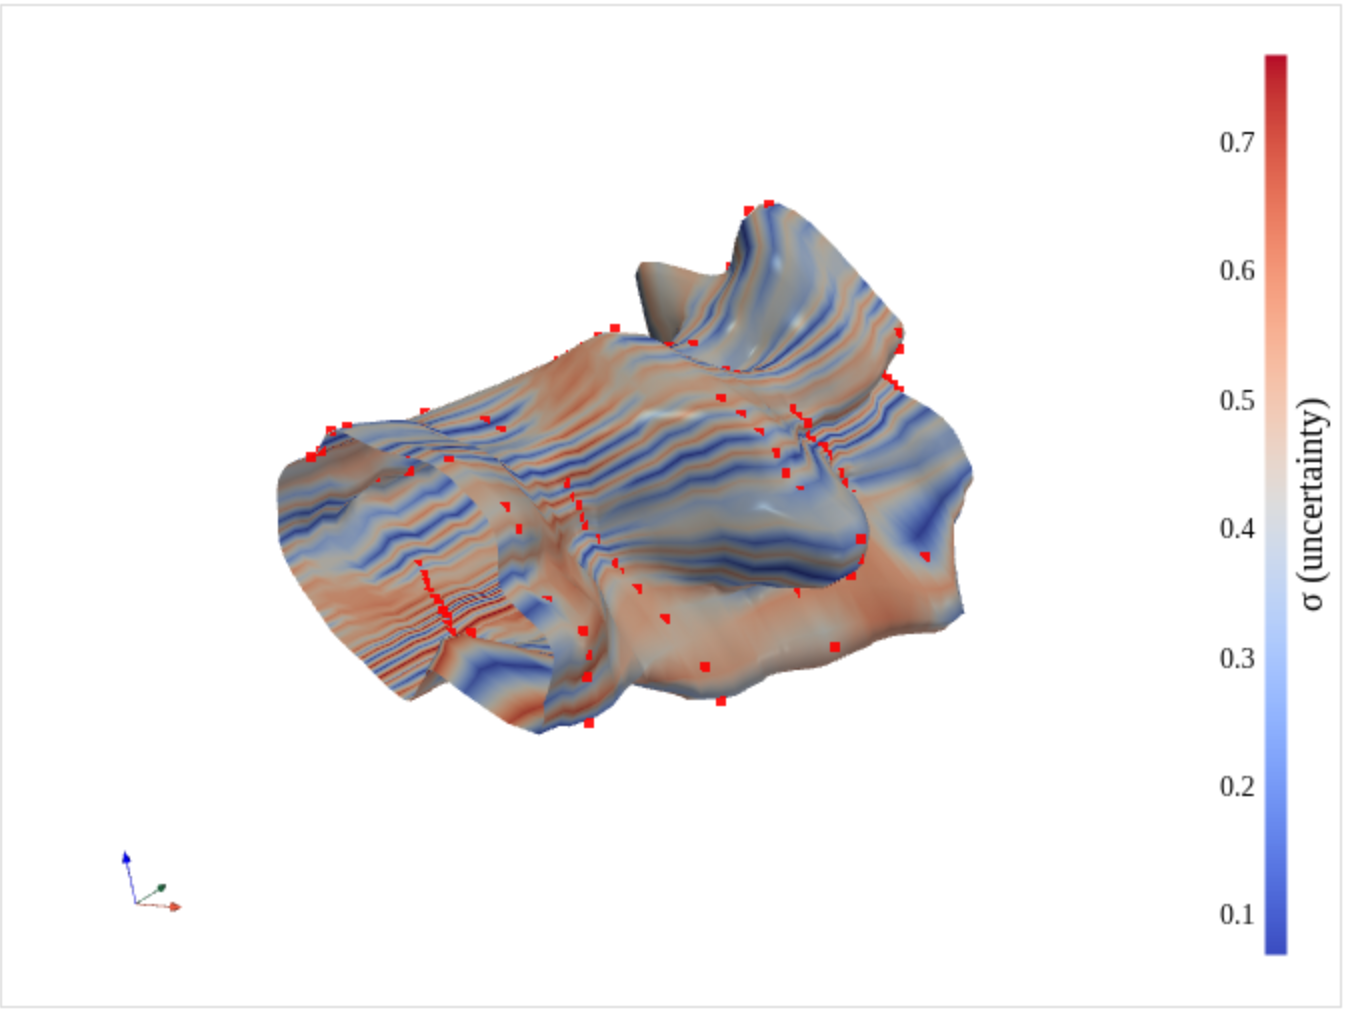
\includegraphics[width=\linewidth]{figures/gp_1.png}\\[0.2em]
    {\small (a)}
  \end{minipage}\hfill
  \begin{minipage}[b]{0.49\linewidth}    % (b) second point of view
    \centering
    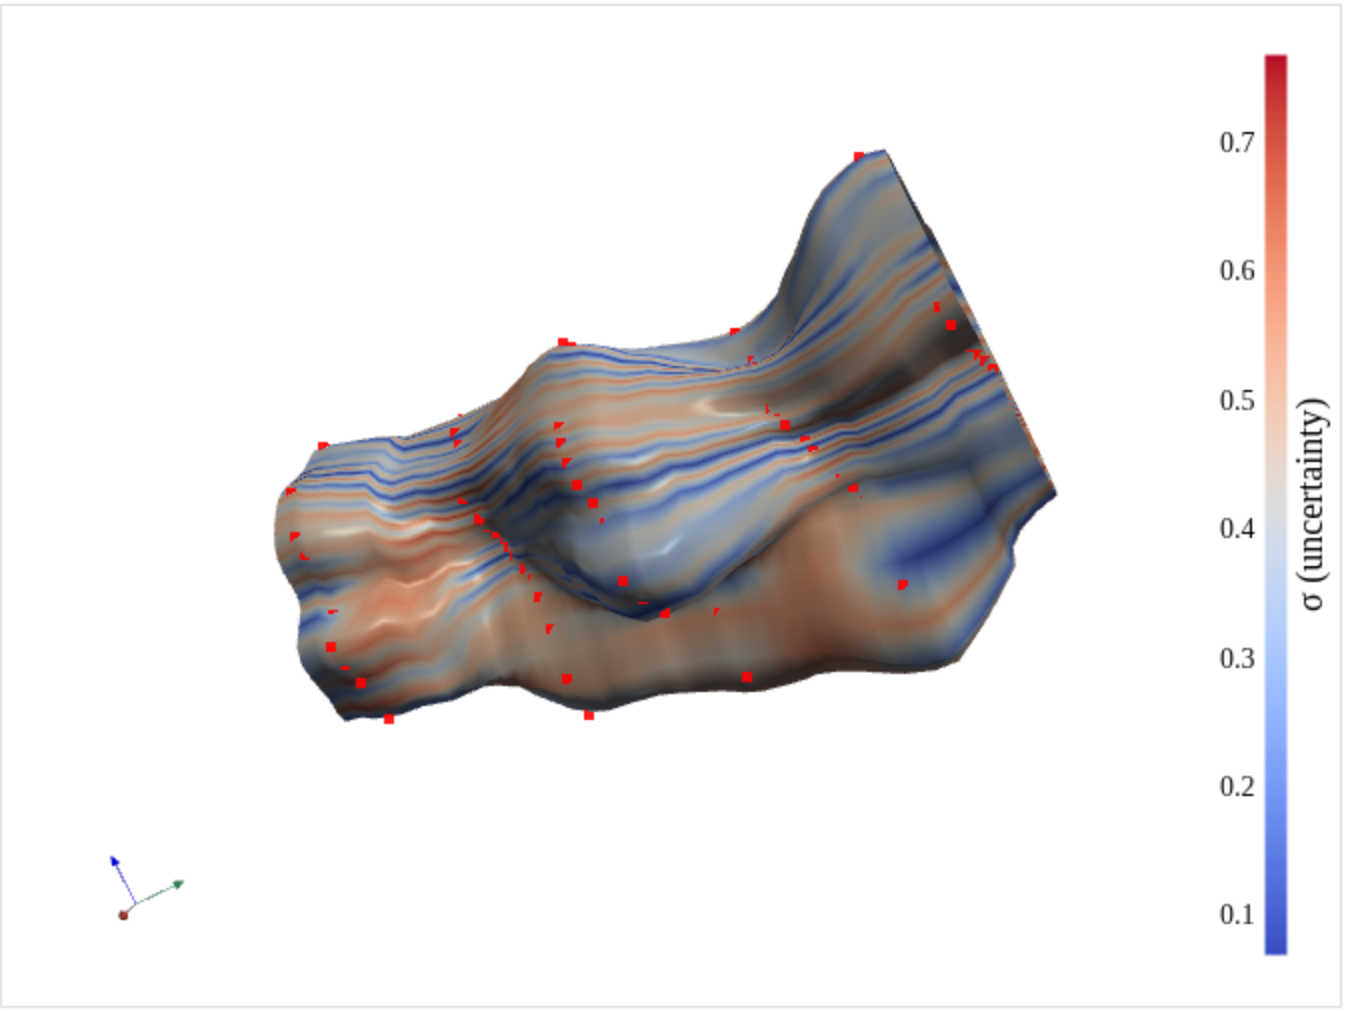
\includegraphics[width=\linewidth]{figures/gp_2.png}\\[0.2em]
    {\small (b)}
  \end{minipage}
  \caption{Surface estimated by the Gaussian process for one scan, shown from two different points of
           view: (a) and (b) are the same surface seen from two viewpoints. The mesh is the predicted
           mean range $\bar{\rho}^{*}(s, \psi^v)$, placed in 3D along the vertical sonar rays, on a
           $40 \times 80$ grid of $(s, \psi^v)$ covering the scan. The colour is the predicted standard
           deviation $\sigma^{*}$ of the range, in metres: blue where the wall is constrained by nearby
           vertical sonar measurements (down to about 0.1~m, the measurement noise), red between and
           away from them (up to about 0.75~m, the prior uncertainty). Red markers: the vertical sonar
           points of the scan, used to train the process.}
  \label{fig:msis_gp_surface}
\end{figure}

% ------------------------------------------------------------------------------
\subsubsection{Maximum likelihood estimation of the elevation angle}  % search inside the beam
\label{sec:msis_mle}                                                  % \secref{sec:msis_mle}

The 3D points observed by the horizontal sonar cannot be obtained directly, since any point in its
beam may return the same measurement. The surface estimated from the vertical sonar is exploited to
infer the elevation angle of each horizontal measurement: elevation angles whose 3D points lie close
to the estimated surface are good estimates (Figure~\ref{fig:msis_mle}). For a horizontal measurement
$(\psi^h_k, \rho^h_k)$ (one echo of $\mathbf{M}^h_k$), the elevation angle is the solution of
\begin{equation}                         % maximum likelihood elevation
  \hat{\theta} = \arg\max_{\theta \in \Theta_H} p\big(\hat{\rho}^v \mid f, \psi^h_k, \rho^h_k,
  \boldsymbol{\eta}_{\sigma^h(k)}, \theta\big)
  = \arg\max_{\theta \in \Theta_H} \ln p\big(\hat{\rho}^v \mid f, \psi^h_k, \rho^h_k,
  \boldsymbol{\eta}_{\sigma^h(k)}, \theta\big)
  = \arg\max_{\theta \in \Theta_H} J(\theta; \psi^h_k, \rho^h_k),
  \label{eq:msis_argmax}
\end{equation}
where $\hat{\rho}^v$ is the range that would have been obtained if this point had been observed by
the vertical sonar. Depending on the environment, several angles can correspond to one measurement
(Figure~\ref{fig:def_frames}b). Instead of the single solution of Eq.~\eqref{eq:msis_argmax}, the
set of local maxima of the log-likelihood is searched:
\begin{equation}                         % set of local maxima
  \hat{\Theta} = \left\{ \hat{\theta} \in \Theta_H \ \middle|\ \frac{\partial J}{\partial\theta}(\hat{\theta}) = 0
  \ \text{and}\ \frac{\partial^2 J}{\partial\theta^2}(\hat{\theta}) < 0 \right\}.
  \label{eq:msis_localmax}
\end{equation}
Since a closed-form expression of the likelihood with respect to $\theta$ is difficult to obtain, the
range $\Theta_H = [-b/2,\, b/2]$, with $b = 25^\circ$ the vertical aperture of the Ping360, is
sampled uniformly with $n_q$ values $\theta_q = -b/2 + q\,\Delta_\theta$, $q \in \{1,\dots,n_q\}$,
$\Delta_\theta = b / n_q$. Each sample gives the virtual 3D point
\begin{equation}                         % candidate point of a sample
  \mathbf{x}(\theta_q) = g^h(\rho^h_k, \theta_q, \psi^h_k, k)
  = \boldsymbol{\eta}_{\sigma^h(k)} \oplus \mathbf{p}_H \oplus
  \begin{bmatrix} \rho^h_k\cos\theta_q\cos\psi^h_k \\ \rho^h_k\cos\theta_q\sin\psi^h_k \\ \rho^h_k\sin\theta_q \end{bmatrix}.
  \label{eq:msis_candidate}
\end{equation}
To assess the likelihood that this point lies on the surface, it must be expressed with the inputs
and output of $f$: the curvilinear abscissa $\hat{s}_q$, the rotation angle $\hat{\psi}^v_q$ and the
range $\hat{\rho}^v_q$ under which the vertical sonar would have seen it
(Figure~\ref{fig:msis_virtual}). This takes the five steps below, detailed in
Algorithm~\ref{alg:msis_mle} (\secref{sec:msis_pseudocode}).

\begin{figure}[!htb]                     % principle of the elevation search
  \centering
  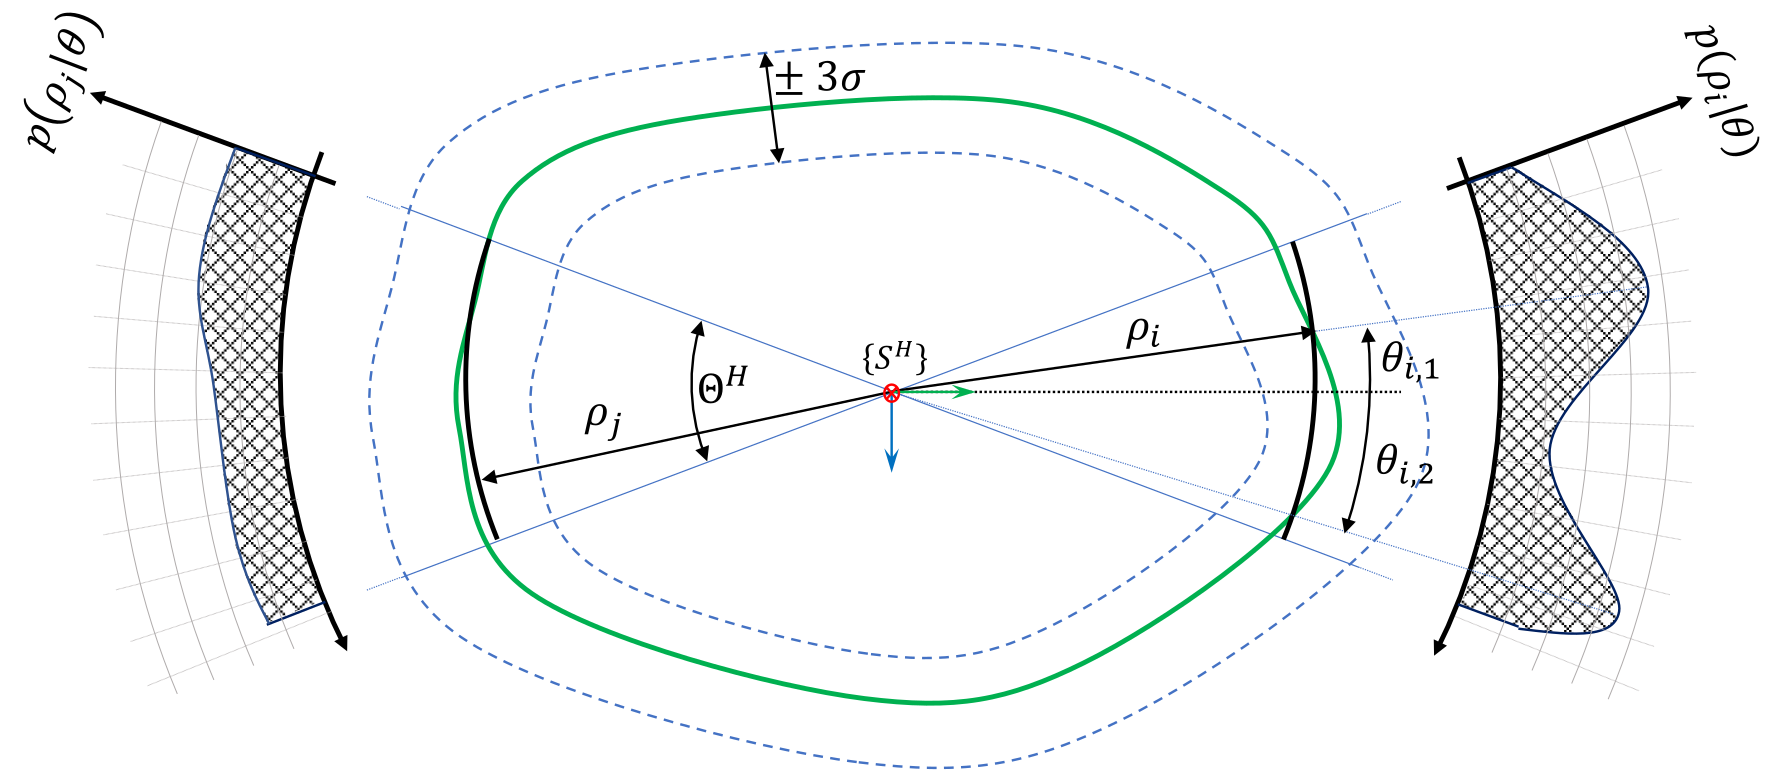
\includegraphics[width=0.85\linewidth, height=7cm, keepaspectratio]{figures/fig_6.png}
  \caption{Principle of the elevation angle estimation on a vertical slice: the elevations whose
           points fall on the estimated surface are the most likely. Adapted from
           \citet{breux2020elevation}.}
  \label{fig:msis_mle}
\end{figure}

\paragraph{1. Selection of the trajectory segments.} Let $\mathbf{n}^v|_{\{S_V\}}$ be the rotation
axis of the vertical sonar expressed in its own frame, which is also the normal of its scanning
plane; since that plane is the $XY$-plane of $\{S_V\}$, $\mathbf{n}^v|_{\{S_V\}} = [0\ 0\ 1]^T$. A pose
$\hat{\boldsymbol{\eta}}_q$ is searched along the trajectory such that $\mathbf{x}(\theta_q)$ belongs
to the vertical sonar plane, which requires interpolating the trajectory. The first step is to
determine the segments of the trajectory that may contain $\hat{\boldsymbol{\eta}}_q$; several
segments can be found. At the $i$-th pose, the rotation axis expressed in the world frame is
\begin{equation}                         % rotation axis of the vertical sonar in {0}
  \mathbf{n}^v|_{\{0\},i} = \mathbf{R}(\mathbf{q}_i)\, \mathbf{R}(\mathbf{q}_V)\, \mathbf{n}^v|_{\{S_V\}},
  \label{eq:msis_axis}
\end{equation}
and the plane passes through the sonar head, at
$\boldsymbol{\tau}^V_i = \boldsymbol{\tau}_i + \mathbf{R}(\mathbf{q}_i)\boldsymbol{\tau}_V$.
\citet{breux2020elevation} measure the distance to the plane from the vehicle origin
$\boldsymbol{\tau}_i$; measuring it from the sonar head matters on the NavScoot~2, whose vertical sonar
is mounted $0.45$~m ahead of the origin, along the normal of its plane
\citep{margaritis2025internship}. A segment $[i, i+1]$ is selected if the projection of
$\mathbf{x}(\theta_q) - \boldsymbol{\tau}^V$ on the rotation axis changes sign between the beginning
and the end of the segment (Figure~\ref{fig:msis_segments}): by the intermediate value theorem, the
segment then contains a pose for which the projection is zero. The set of starting indices is
\begin{equation}                         % segments crossing the plane
  I_q = \Big\{ i \ \Big|\ \big\langle \mathbf{n}^v|_{\{0\},i},\, \mathbf{x}(\theta_q) - \boldsymbol{\tau}^V_i \big\rangle
  \big\langle \mathbf{n}^v|_{\{0\},i+1},\, \mathbf{x}(\theta_q) - \boldsymbol{\tau}^V_{i+1} \big\rangle < 0 \Big\}.
  \label{eq:msis_segments}
\end{equation}

\paragraph{2. Interpolation of the pose.} For each selected segment, $\boldsymbol{\eta}_{[i,i+1]} :
[0, 1] \to SE(3)$ denotes the linear interpolation between the poses $\boldsymbol{\eta}_i$ and
$\boldsymbol{\eta}_{i+1}$. Its position is
\begin{equation}                         % interpolated position
  \boldsymbol{\tau}_{[i,i+1]}(t) = (\boldsymbol{\tau}_{i+1} - \boldsymbol{\tau}_i)\, t + \boldsymbol{\tau}_i.
  \label{eq:msis_interp_pos}
\end{equation}
For the orientation, the relative rotation between the two poses is expressed by its yaw, pitch and
roll Euler angles,
\begin{equation}                         % relative rotation between consecutive poses
  [\delta\psi\ \ \delta\chi\ \ \delta\phi]^T = \operatorname{Euler}\big(\mathbf{R}(\mathbf{q}_i)^T \mathbf{R}(\mathbf{q}_{i+1})\big),
  \label{eq:msis_euler}
\end{equation}
which is the rotational part of $\boldsymbol{\eta}_{i+1} \ominus \boldsymbol{\eta}_i$. The interpolated
rotation, the global rotation and the interpolated rotation axis of the vertical sonar are
\begin{align}                            % interpolated rotation and axis
  \delta\mathbf{R}(t) &= \mathbf{R}(\delta\psi\, t, \delta\chi\, t, \delta\phi\, t),                 \label{eq:msis_deltaR}\\
  \mathbf{R}(t)       &= \mathbf{R}(\mathbf{q}_i)\, \delta\mathbf{R}(t),                              \label{eq:msis_Rt}\\
  \mathbf{n}^v|_{\{0\},[i,i+1]}(t) &= \mathbf{R}(t)\, \mathbf{R}(\mathbf{q}_V)\, \mathbf{n}^v|_{\{S_V\}}, \label{eq:msis_axis_t}
\end{align}
and the interpolated sonar head is
$\boldsymbol{\tau}^V_{[i,i+1]}(t) = \boldsymbol{\tau}_{[i,i+1]}(t) + \mathbf{R}(t)\boldsymbol{\tau}_V$.
The interpolation value $\hat{t}$ is the one for which $\mathbf{x}(\theta_q)$ belongs to the sonar
plane of normal $\mathbf{n}^v|_{\{0\},[i,i+1]}(\hat{t})$:
\begin{equation}                         % crossing condition
  \big\langle \mathbf{n}^v|_{\{0\},[i,i+1]}(\hat{t}),\ \mathbf{x}(\theta_q) - \boldsymbol{\tau}^V_{[i,i+1]}(\hat{t}) \big\rangle = 0.
  \label{eq:msis_plane}
\end{equation}
Assuming small angle variations between consecutive poses, $\delta\mathbf{R}$ is approximated to the
first order:
\begin{equation}                         % first-order rotation
  \delta\mathbf{R}(t) \approx
  \begin{bmatrix} 1 & -\delta\psi\, t & \delta\chi\, t \\ \delta\psi\, t & 1 & -\delta\phi\, t \\ -\delta\chi\, t & \delta\phi\, t & 1 \end{bmatrix}
  = \mathbf{I}_3 + t\,[\delta\boldsymbol{\omega}]_\times, \qquad
  \delta\boldsymbol{\omega} = [\delta\phi\ \ \delta\chi\ \ \delta\psi]^T.
  \label{eq:msis_firstorder}
\end{equation}
Written in the frame of the vertical sonar, i.e.\ as the coordinate of $\mathbf{x}(\theta_q)$ along
$\mathbf{n}^v|_{\{S_V\}}$ in $\{S_V\}$, Eq.~\eqref{eq:msis_plane} then becomes a polynomial equation
of degree two in $\hat{t}$:
\begin{equation}                         % crossing condition as a quadratic
  \mathbf{n}^{v}|_{\{S_V\}}^T\, \mathbf{R}(\mathbf{q}_V)^T \Big( \delta\mathbf{R}(\hat{t})^T\,
  \mathbf{R}(\mathbf{q}_i)^T \big( (\boldsymbol{\tau}_i - \boldsymbol{\tau}_{i+1})\, \hat{t} + \mathbf{x}(\theta_q) -
  \boldsymbol{\tau}_i \big) - \boldsymbol{\tau}_V \Big) = 0.
  \label{eq:msis_quadratic}
\end{equation}
With $\mathbf{m} = \mathbf{R}(\mathbf{q}_V)\mathbf{n}^v|_{\{S_V\}}$ the axis in the body frame,
$\mathbf{a} = \mathbf{R}(\mathbf{q}_i)^T(\mathbf{x}(\theta_q) - \boldsymbol{\tau}_i)$ and
$\mathbf{d} = \mathbf{R}(\mathbf{q}_i)^T(\boldsymbol{\tau}_{i+1} - \boldsymbol{\tau}_i)$, its coefficients
are
\begin{equation}                         % coefficients of the quadratic
  c_2 \hat{t}^2 + c_1 \hat{t} + c_0 = 0, \qquad
  c_2 = \mathbf{m}^T [\delta\boldsymbol{\omega}]_\times \mathbf{d}, \quad
  c_1 = -\mathbf{m}^T \big(\mathbf{d} + [\delta\boldsymbol{\omega}]_\times \mathbf{a}\big), \quad
  c_0 = \mathbf{m}^T (\mathbf{a} - \boldsymbol{\tau}_V).
  \label{eq:msis_coeffs}
\end{equation}
$c_0$ is the signed distance to the plane at $\boldsymbol{\eta}_i$ and $c_2$ is small, being the
product of the rotation increment and the displacement, so the equation has a single root in
$[0, 1]$ (it is linear if $c_2 = 0$). The interpolated pose
$\hat{\boldsymbol{\eta}}_q = \boldsymbol{\eta}_{[i,i+1]}(\hat{t})$ uses the exact rotation of
Eqs.~\eqref{eq:msis_deltaR}--\eqref{eq:msis_Rt}; the first-order approximation only serves to find
$\hat{t}$.

\begin{figure}[!htb]                     % geometry of the virtual vertical measurement
  \centering
  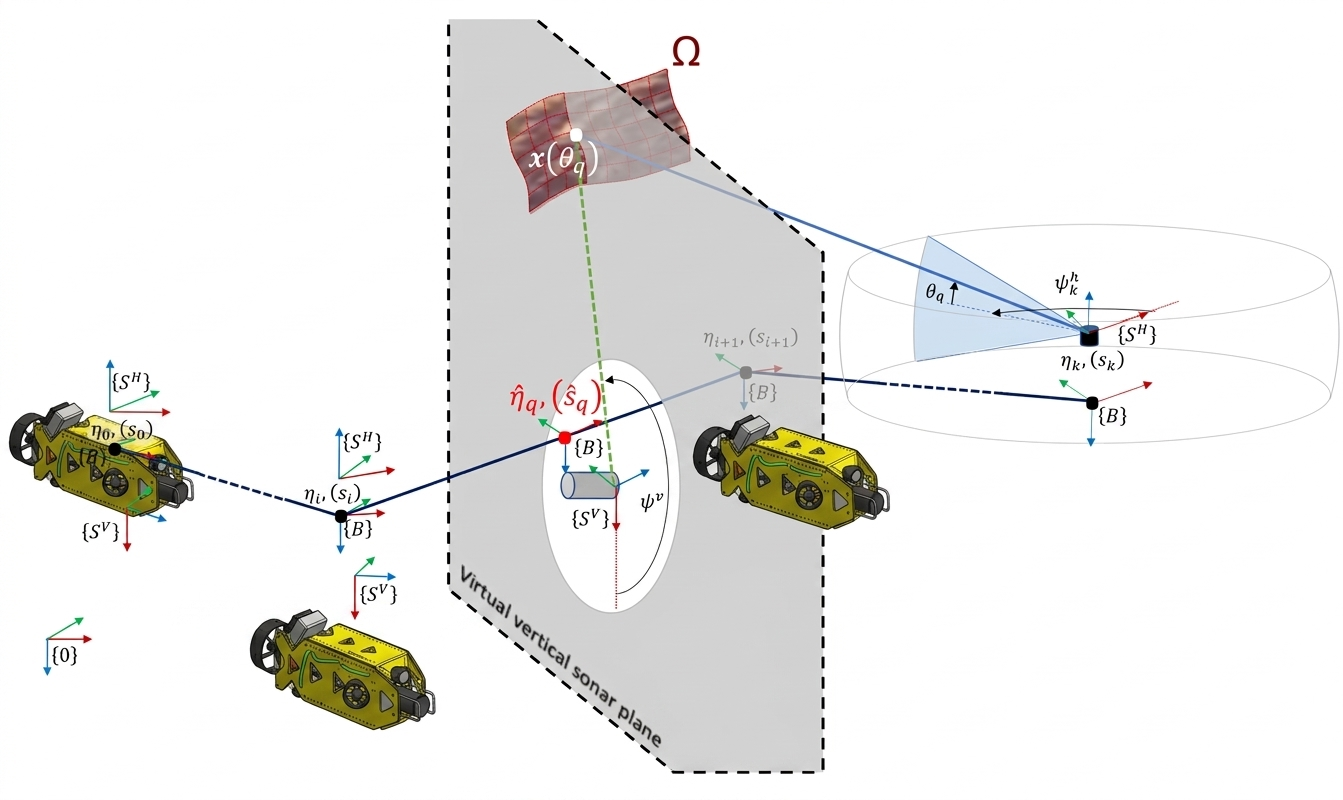
\includegraphics[width=0.85\linewidth, height=7cm, keepaspectratio]{figures/fig_7.jpeg}
  \caption{Virtual vertical measurement of a candidate point seen by the horizontal sonar. Adapted
           from \citet{breux2020elevation}.}
  \label{fig:msis_virtual}
\end{figure}

\begin{figure}[!htb]                     % segment selection
  \centering
  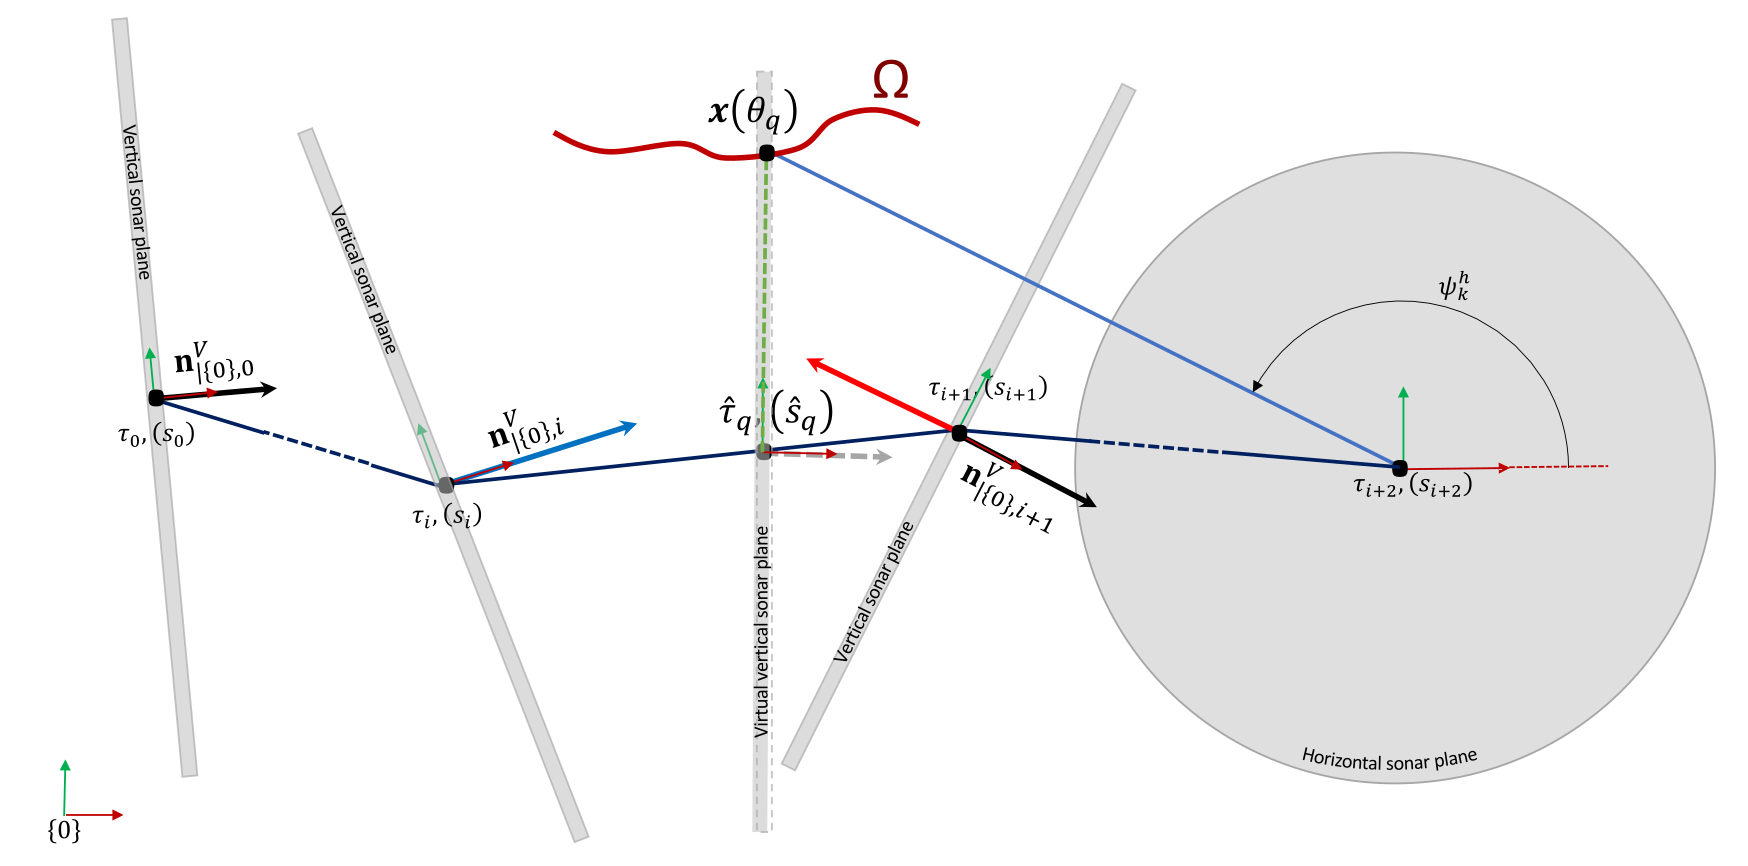
\includegraphics[width=0.85\linewidth, height=7cm, keepaspectratio]{figures/fig_8.png}
  \caption{Selection of the trajectory segment containing the pose of the virtual measurement.
           Adapted from \citet{breux2020elevation}.}
  \label{fig:msis_segments}
\end{figure}

\paragraph{3. Virtual vertical measurement.} The curvilinear abscissa corresponding to $\hat{t}$ is
\begin{equation}                         % abscissa of the virtual measurement
  \hat{s}_q = s_i + L_{\boldsymbol{\eta}_i}^{\hat{\boldsymbol{\eta}}_q}
            = s_i + \big\lVert \log(\mathbf{T}_i^{-1}\hat{\mathbf{T}}_q) \big\rVert_G,
  \label{eq:msis_shat}
\end{equation}
with $\hat{\mathbf{T}}_q$ the matrix of $\hat{\boldsymbol{\eta}}_q$. To compute $\hat{\psi}^v_q$,
$\mathbf{x}(\theta_q)$ is expressed in the frame of the vertical sonar at the pose
$\hat{\boldsymbol{\eta}}_q$, where its third coordinate is zero by construction of $\hat{t}$:
\begin{align}                            % virtual vertical measurement
  \hat{\mathbf{x}}(\theta_q)|_{\{S_V\}} &= \mathbf{x}(\theta_q) \ominus (\hat{\boldsymbol{\eta}}_q \oplus \mathbf{p}_V)
                                        = [\hat{x}^v\ \ \hat{y}^v\ \ 0]^T,                  \label{eq:msis_xhat}\\
  \hat{\psi}^v_q &= \operatorname{atan2}(\hat{y}^v, \hat{x}^v),                             \label{eq:msis_psihat}\\
  \hat{\rho}^v_q &= \big\lVert \hat{\mathbf{x}}(\theta_q)|_{\{S_V\}} \big\rVert_2.          \label{eq:msis_rhohat}
\end{align}

\paragraph{4. Log-likelihood.} The Gaussian process trained to estimate $f$ predicts, at the input
$(\hat{s}_q, \hat{\psi}^v_q)$ and with the prior $f_p(\hat{\boldsymbol{\eta}}_q, \hat{\psi}^v_q)$, the
range (Eqs.~\eqref{eq:def_gp_mean}--\eqref{eq:def_gp_var}, \citealt[Eqs.~2.25--2.26]{rasmussen2006gaussian})
\begin{equation}                         % GP prediction at the virtual input
  \rho^{*}_q \sim \mathcal{N}\big(\bar{\rho}^{*}_q, \sigma^{*2}_q\big),
  \label{eq:msis_gppred}
\end{equation}
and the log-likelihood of the virtual range is
\begin{equation}                         % Gaussian log-likelihood
  J(\theta_q; \psi^h_k, \rho^h_k) = \ln p\big(\hat{\rho}^v_q \mid f, \psi^h_k, \rho^h_k,
  \boldsymbol{\eta}_{\sigma^h(k)}, \theta_q\big)
  = -\left( \frac{(\bar{\rho}^{*}_q - \hat{\rho}^v_q)^2}{2\sigma^{*2}_q} + \ln \sigma^{*}_q + \frac{\ln(2\pi)}{2} \right).
  \label{eq:msis_loglik}
\end{equation}
If the trajectory crosses the plane in several segments, the most likely crossing is kept. If no
segment is found, $\mathbf{x}(\theta_q)$ lies outside the part of the conduit swept by the vertical
sonar during the scan: the sample gets $J = -\infty$ and cannot be a maximum.

\paragraph{5. Local maxima.} Eq.~\eqref{eq:msis_localmax} is evaluated on the samples: $\theta_{q-1}$
is kept when its log-likelihood is larger than those of its two neighbours $\theta_{q-2}$ and
$\theta_q$, which approximates $\partial J / \partial\theta = 0$ and $\partial^2 J / \partial\theta^2 < 0$.
The resolution of the estimates is therefore $\Delta_\theta = b / n_q$.

% ------------------------------------------------------------------------------
\FloatBarrier                            % print the figures of 4.2.3 before 4.2.4 starts
\subsubsection{Estimation uncertainty}   % scaled beta distribution of each estimate
\label{sec:msis_uncertainty}             % \secref{sec:msis_uncertainty}

Each estimated angle $\hat{\theta} \in \hat{\Theta}$ also needs an uncertainty, i.e.\ a probability
distribution $p(\hat{\theta})$. A normal distribution is not adapted, as its support is infinite while
the angle is restricted to the aperture of the beam. A good choice is the scaled beta distribution
\citep{johnson1994continuous} of Eq.~\eqref{eq:def_beta}, defined by two parameters $\alpha$, $\beta$,
\begin{equation}                         % scaled beta distribution of an estimate
  \hat{\theta} \sim \operatorname{Beta}(\alpha, \beta, \theta_{\min}, \theta_{\max}), \qquad
  \theta_{\max} = -\theta_{\min} = \frac{b}{2},
  \label{eq:msis_beta}
\end{equation}
whose density involves the gamma function of Eq.~\eqref{eq:def_gamma} and whose parameters follow
from a mean $\bar{\theta}$ and a variance $\sigma_\theta^2$ through Eq.~\eqref{eq:def_beta_params}. The
mean is simply the estimate, $\bar{\theta} = \hat{\theta}$. The variance is estimated as the inverse of
the Fisher information $\mathcal{I}(\bar{\theta})$:
\begin{equation}                         % variance from the Fisher information
  \sigma_\theta^2 = \frac{1}{\mathcal{I}(\bar{\theta})}, \qquad
  \mathcal{I}(\theta) = -\mathbb{E}\!\left[\frac{\partial^2 \ln p(\rho^v \mid \theta)}{\partial\theta^2} \,\middle|\, \theta\right]
  = -\int \frac{\partial^2 \ln p(\rho^v \mid \theta)}{\partial\theta^2}\, p(\rho^v \mid \theta)\, d\rho^v.
  \label{eq:msis_fisher}
\end{equation}
The likelihood is the Gaussian prediction of the process at the virtual input of $\theta$,
$p(\rho^v \mid \theta) = \mathcal{N}\big(\bar{\rho}(\theta), \sigma_\rho^2(\theta)\big)$, with
$\bar{\rho} = \bar{\rho}^{*}$ and $\sigma_\rho = \sigma^{*}$ of Eq.~\eqref{eq:msis_gppred}. Direct
computation of Eq.~\eqref{eq:msis_fisher} then gives
\begin{equation}                         % closed-form variance
  \sigma_\theta^2 = \frac{\sigma_\rho^2(\bar{\theta})}
  {2\left(\left.\dfrac{\partial\sigma_\rho}{\partial\theta}\right|_{\bar{\theta}}\right)^2
   + \left(\left.\dfrac{\partial\bar{\rho}}{\partial\theta}\right|_{\bar{\theta}}\right)^2}.
  \label{eq:msis_sigmatheta}
\end{equation}
An angle is therefore well determined when a small change of $\theta$ moves the predicted range or
its uncertainty by much more than that uncertainty.

\paragraph{Derivation of the Fisher information.} Following Appendix~A of \citet{breux2020elevation},
write $\bar{\rho}$, $\sigma$ for $\bar{\rho}(\theta)$, $\sigma_\rho(\theta)$, primes for derivatives with
respect to $\theta$, and $u = \rho^v - \bar{\rho}$. The negative log-likelihood and its first two
derivatives are
\begin{align}                            % derivation of the Fisher information
  -\ln p(\rho^v \mid \theta) &= \ln\sigma + \frac{\ln 2\pi}{2} + \frac{u^2}{2\sigma^2},              \label{eq:msis_A1}\\
  -\frac{\partial \ln p(\rho^v \mid \theta)}{\partial\theta}
    &= \frac{\sigma'}{\sigma} - \frac{u\,\bar{\rho}'}{\sigma^2} - \frac{u^2\sigma'}{\sigma^3},        \label{eq:msis_A2}\\
  -\frac{\partial^2 \ln p(\rho^v \mid \theta)}{\partial\theta^2}
    &= \frac{\sigma\sigma'' - \sigma'^2}{\sigma^2} + \frac{\bar{\rho}'^2}{\sigma^2} - \frac{u\,\bar{\rho}''}{\sigma^2}
       + \frac{4u\,\bar{\rho}'\sigma'}{\sigma^3} - \frac{u^2(\sigma\sigma'' - 3\sigma'^2)}{\sigma^4}.   \label{eq:msis_A3}
\end{align}
Taking the expectation with $\mathbb{E}[u] = 0$ and $\mathbb{E}[u^2] = \sigma^2$, the terms in $\sigma''$
cancel and
\begin{equation}                         % Fisher information of a Gaussian likelihood
  \mathcal{I}(\theta) = \frac{2\sigma'^2 + \bar{\rho}'^2}{\sigma^2},
  \label{eq:msis_A5}
\end{equation}
which is Eq.~\eqref{eq:msis_sigmatheta}. In practice the derivatives are evaluated by central finite
differences on the samples $\theta_q$ of Algorithm~\ref{alg:msis_mle} (one-sided differences when a
neighbouring sample has no crossing). When both sonars are at the same place, as in Fig.~6 of
\citet{breux2020elevation}, the virtual range $\hat{\rho}^v$ does not depend on $\theta$. On the
NavScoot~2 the two sonars are about $0.3$~m apart, so $\hat{\rho}^v$ varies slightly with $\theta$;
using the derivative of the residual $\bar{\rho}^{*} - \hat{\rho}^v$ in place of $\bar{\rho}'$ accounts
for this.

\paragraph{Validity thresholds.} A uniform distribution is still a beta distribution, with
$\alpha = \beta = 1$: from Eqs.~\eqref{eq:def_beta} and \eqref{eq:def_gamma},
\begin{equation}                         % uniform as a beta distribution
  p(\theta; 1, 1, b) = \frac{\Gamma(2)}{b\,\Gamma(1)\,\Gamma(1)} = \frac{1}{b},
  \label{eq:msis_uniform}
\end{equation}
the density of the uniform distribution on $[-b/2,\, b/2]$. A threshold $\sigma_l$ is defined to filter
out the variances $\sigma_\theta$ that lead to invalid beta parameters. First, $\alpha$ and $\beta$ must
be strictly positive:
\begin{equation}                         % positivity of the parameters
  \alpha > 0,\ \beta > 0 \iff \sigma_\theta^2 < \left(\frac{b}{2}\right)^2 - \bar{\theta}^2.
  \label{eq:msis_valid}
\end{equation}
Furthermore, each distribution is assumed unimodal, so $\alpha \geq 1$ or $\beta \geq 1$: if
$\alpha, \beta < 1$, the distribution is U-shaped, with its modes at the edges $\pm b/2$ of the beam.
From Eq.~\eqref{eq:def_beta_params},
\begin{align}                            % unimodality conditions
  \alpha \geq 1 &\iff \sigma_\theta^2 \leq A(\bar{\theta}) = \frac{(b + 2\bar{\theta})^2 (b - 2\bar{\theta})}{4(3b + 2\bar{\theta})}, \label{eq:msis_alpha1}\\
  \beta \geq 1  &\iff \sigma_\theta^2 \leq B(\bar{\theta}) = A(-\bar{\theta}),                                                   \label{eq:msis_beta1}
\end{align}
which implies
\begin{equation}                         % unimodality threshold
  \sigma_\theta^2 \leq \sigma_l^2(\bar{\theta}) = \max\big(A(\bar{\theta}), A(-\bar{\theta})\big) = A(|\bar{\theta}|).
  \label{eq:msis_sigmal}
\end{equation}
The first constraint is included in the second, since
$A(|\bar{\theta}|) = \big((b/2)^2 - \bar{\theta}^2\big)\,(b + 2|\bar{\theta}|)/(3b + 2|\bar{\theta}|)$, so that
\begin{equation}                         % inclusion of the constraints
  \forall \bar{\theta} \in \left[-\frac{b}{2}, \frac{b}{2}\right], \quad
  \sigma_l^2(\bar{\theta}) = A(|\bar{\theta}|) \leq \left(\frac{b}{2}\right)^2 - \bar{\theta}^2.
  \label{eq:msis_incl}
\end{equation}
A second threshold $\sigma_m$ filters out estimations that are valid but too uncertain:
\begin{equation}                         % maximum uncertainty
  k\,\sigma_m = \frac{b}{2},
  \label{eq:msis_sigmam}
\end{equation}
where the parameter $k$ controls the sensitivity of the filter, higher values being more
restrictive; \citet{breux2020elevation} use $k = 3$ by default. The final threshold is
\begin{equation}                         % final threshold
  \sigma_T^2(\bar{\theta}) = \min\big(\sigma_l^2(\bar{\theta}),\ \sigma_m^2\big).
  \label{eq:msis_sigmaT}
\end{equation}
If $\sigma_\theta \leq \sigma_T$, $\alpha$ and $\beta$ are computed with Eq.~\eqref{eq:def_beta_params};
otherwise the estimate carries no reliable information and its distribution is the uniform one.
Figure~\ref{fig:msis_thresholds} shows these thresholds for the Ping360 ($b = 25^\circ$) and $k = 3$:
$\sigma_m \approx 4.2^\circ$, while $\sigma_l$ equals the standard deviation of the uniform
distribution, $b/\sqrt{12} \approx 7.2^\circ$, at the centre of the beam, peaks at $7.5^\circ$ for
$|\bar{\theta}| \approx 3^\circ$ and drops to zero at the edges. Hence $\sigma_T = \sigma_m$ for
$|\bar{\theta}| \leq 11^\circ$, and $\sigma_T = \sigma_l$ in the last $1.5^\circ$ of each side of the beam.

\begin{figure}[!htb]                     % thresholds computed for the Ping360
  \centering
  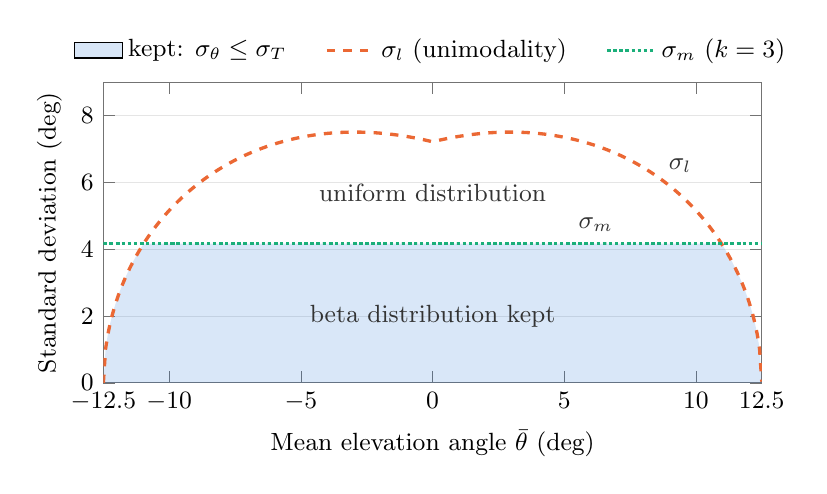
\begin{tikzpicture}
    \begin{axis}[
        width=0.82\linewidth, height=5.4cm,
        xmin=-12.5, xmax=12.5, ymin=0, ymax=9,
        xtick={-12.5,-10,-5,0,5,10,12.5},
        ytick={0,2,4,6,8},
        xlabel={Mean elevation angle $\bar{\theta}$ (deg)},
        ylabel={Standard deviation (deg)},
        ymajorgrids, grid style={black!10},
        axis line style={black!55}, tick style={black!55},
        tick label style={font=\small}, label style={font=\small},
        legend style={at={(0.5,1.03)}, anchor=south, legend columns=3, draw=none, font=\small,
                      /tikz/every even column/.append style={column sep=1.2em}},
        legend cell align=left,
        domain=-12.5:12.5, samples=301,
      ]
      \addplot[draw=none, fill=vizBlue, fill opacity=0.18, area legend]
        {min(sqrt(max((25 + 2*abs(x))^2*(25 - 2*abs(x))/(4*(75 + 2*abs(x))), 0)), 25/6)} \closedcycle;
      \addlegendentry{kept: $\sigma_\theta \leq \sigma_T$}
      \addplot[vizOrange, line width=1.2pt, dashed]
        {sqrt(max((25 + 2*abs(x))^2*(25 - 2*abs(x))/(4*(75 + 2*abs(x))), 0))};
      \addlegendentry{$\sigma_l$ (unimodality)}
      \addplot[vizAqua, line width=1.2pt, densely dotted] {25/6};
      \addlegendentry{$\sigma_m$ ($k = 3$)}
      \node[font=\small, text=black!80] at (axis cs:0,2)      {beta distribution kept};
      \node[font=\small, text=black!80] at (axis cs:0,5.7)    {uniform distribution};
      \node[font=\small, text=black!80, anchor=west] at (axis cs:8.6,6.5)  {$\sigma_l$};
      \node[font=\small, text=black!80, anchor=south] at (axis cs:6.2,4.25) {$\sigma_m$};
    \end{axis}
  \end{tikzpicture}
  \caption{Thresholds on the standard deviation $\sigma_\theta$ of an elevation estimate as a function
           of its mean $\bar{\theta}$, for the Ping360 ($b = 25^\circ$) and $k = 3$, computed from
           Eqs.~\eqref{eq:msis_sigmal}--\eqref{eq:msis_sigmaT}. Estimates below
           $\sigma_T = \min(\sigma_l, \sigma_m)$ (shaded) keep their beta distribution; the others are
           replaced by the uniform distribution. Fig.~9 of \citet{breux2020elevation} shows the same
           thresholds, as variances, for a $35^\circ$ beam.}
  \label{fig:msis_thresholds}
\end{figure}

To display the result, \citet{breux2020elevation} colour the measured arc of each echo with the
density of its beta distributions, through the mapping
\begin{equation}                         % colour mapping of densities
  m : \left\{
  \begin{array}{rcl}
    \mathbb{R}^+ & \to     & [0, 1] \\
    x            & \mapsto & \dfrac{2}{\pi}\arctan(b x)
  \end{array}\right.
  \label{eq:msis_colour}
\end{equation}
whose central colour, $m = 1/2$, is obtained for $x = 1/b$, the density of the uniform distribution
(Figure~\ref{fig:msis_uncertainty}). Algorithm~\ref{alg:msis_uncertainty} (\secref{sec:msis_pseudocode})
summarizes the computation of the distribution of one estimate.

\begin{figure}[!htb]                     % uncertainty of one echo
  \centering
  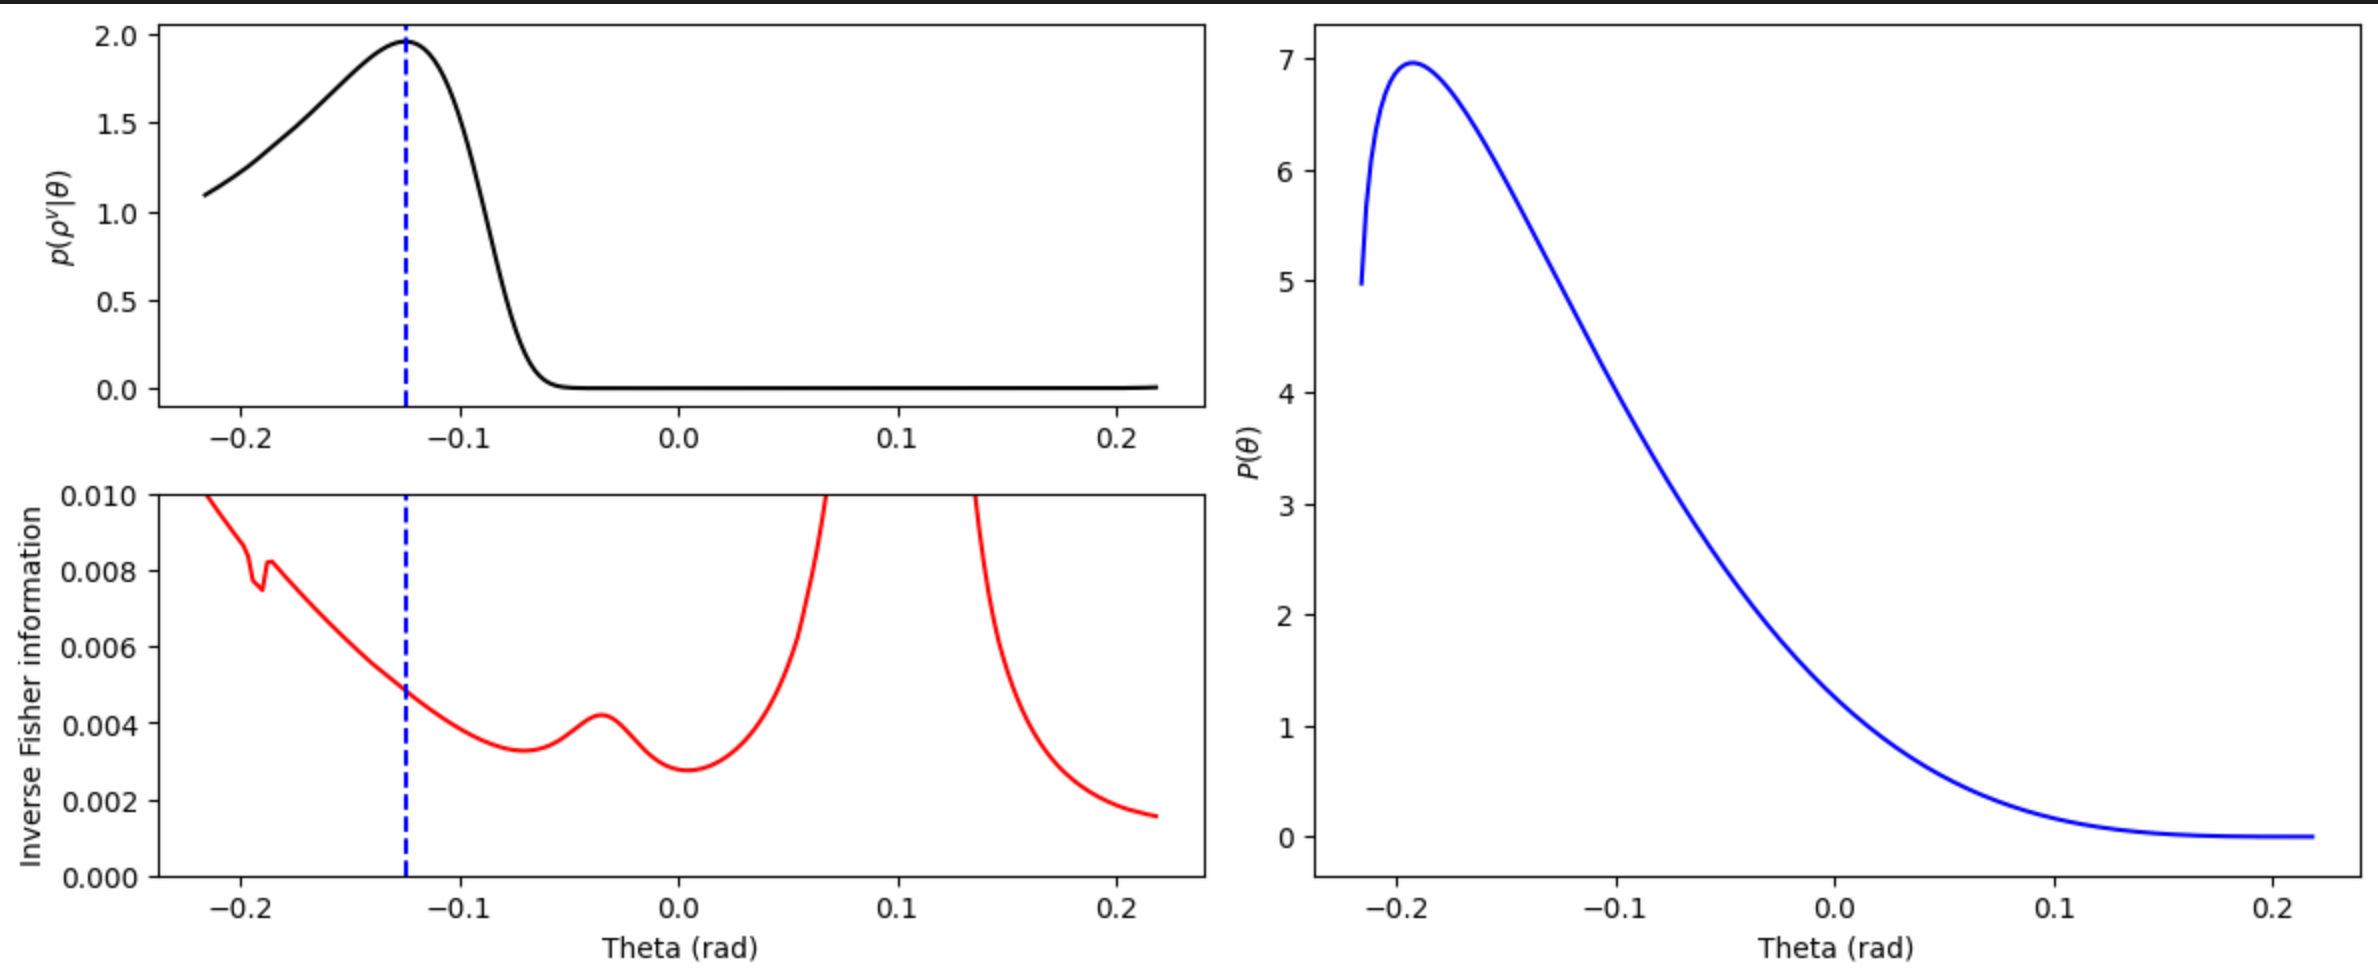
\includegraphics[width=\linewidth]{figures/diagrams.png}
  \caption{Uncertainty estimation for one echo of the horizontal sonar, over its whole vertical
           aperture $\theta \in [-b/2,\, b/2]$ ($b = 25^\circ \approx 0.44$~rad).
           \emph{Top left:} likelihood $p(\rho^v \mid \theta)$ of each candidate elevation angle,
           i.e.\ how well the 3D point given by $\theta$ falls on the surface estimated by the
           Gaussian process (Eq.~\eqref{eq:msis_loglik}). It has a single local maximum,
           $\bar{\theta} \approx -0.125$~rad (dashed blue line); for $\theta > -0.05$~rad the points
           fall far from the surface and the likelihood vanishes.
           \emph{Bottom left:} inverse Fisher information $1/\mathcal{I}(\theta)$, i.e.\ the variance
           $\sigma_\theta^2$ an estimate would have at each $\theta$ (Eq.~\eqref{eq:msis_sigmatheta}).
           It is small where the likelihood changes quickly with $\theta$ and grows without bound where
           the likelihood is flat (around $0.1$~rad). At $\bar{\theta}$ it is about
           $0.0048$~rad$^2$, i.e.\ $\sigma_\theta \approx 0.07$~rad, just below the threshold
           $\sigma_T = \sigma_m \approx 0.073$~rad, so the estimate is kept.
           \emph{Right:} resulting scaled beta distribution $p(\theta)$ of the estimate
           (Eq.~\eqref{eq:def_beta}), with mean $\bar{\theta}$ and variance $\sigma_\theta^2$
           ($\alpha \approx 1.2$, $\beta \approx 4.4$). Because $\bar{\theta}$ is close to the lower
           edge of the beam and the distribution cannot extend beyond it, it is skewed: its peak
           ($\approx -0.19$~rad) lies closer to the edge than its mean.}
  \label{fig:msis_uncertainty}
\end{figure}

% \hint{Add the settings used on the NavScoot~2 data: how the echoes are extracted from the Ping360
% intensity profiles, how the recording is cut into complete scans, the kernels and hyperparameters
% chosen, the number of samples $n_q$ and the threshold $k$.}

% ==============================================================================
\clearpage                               % the pseudocode starts on its own page
\subsection{Pseudocode}                  % the three algorithms, always kept together here
\label{sec:msis_pseudocode}              % \secref{sec:msis_pseudocode}

Algorithms~\ref{alg:msis_merging} to \ref{alg:msis_uncertainty} give the complete pseudocode of the
method: the scan merging (Algorithm~\ref{alg:msis_merging}), the maximum likelihood estimation of the
elevation angles (Algorithm~\ref{alg:msis_mle}, \secref{sec:msis_mle}) and the estimation of their
uncertainty (Algorithm~\ref{alg:msis_uncertainty}, \secref{sec:msis_uncertainty}). The line numbers
quoted in the text refer to these algorithms.

\begin{algorithm}[H]                     % Algorithm 1 of Breux and Lapierre (2020), written out
  \caption{Scan merging \citep{breux2020elevation}.}
  \label{alg:msis_merging}
  \small                                 % slightly smaller so the three algorithms fit on two pages
  \begin{algorithmic}[1]
    \Require Horizontal measurements $\mathcal{M}^h = \{\mathbf{M}^h_k\}_{k=1}^{n_h}$ and vertical
             measurements $\mathcal{M}^v = \{\mathbf{m}^v_k\}_{k=1}^{n_v}$ of one complete scan;
             trajectory $\mathcal{H} = \{\boldsymbol{\eta}_i\}_{i=1}^{n_r}$; sonar poses
             $\mathbf{p}_H$, $\mathbf{p}_V$; beam aperture $b$
    \Ensure Distributions $p(\hat{\theta})$ of the elevation angles of every horizontal echo;
            merged point cloud $\mathcal{P}$
    \Statex $\triangleright$ \textit{Curvilinear abscissa}
    \State $s_1 \gets 0$
    \For{$i = 2, \dots, n_r$}
      \State $\boldsymbol{\xi}_i \gets \log(\mathbf{T}_{i-1}^{-1}\mathbf{T}_i)$
             \Comment{Relative motion}
      \State $s_i \gets s_{i-1} + \sqrt{\boldsymbol{\xi}_i^T \mathbf{G}\, \boldsymbol{\xi}_i}$
             \Comment{Eq.~\eqref{eq:msis_abscissa}}
    \EndFor
    \Statex $\triangleright$ \textit{Environment prior}
    \State $\mathcal{P}^v \gets \{ g^v(\rho^v_k, 0, \psi^v_k, k) \mid \mathbf{m}^v_k \in \mathcal{M}^v \}$
           \Comment{Vertical sonar points in $\{0\}$}
    \State $f_p \gets \Call{FitEllipticCylinder}{\mathcal{P}^v}$
           \Comment{Eqs.~\eqref{eq:msis_prior}--\eqref{eq:msis_lm}}
    \Statex $\triangleright$ \textit{Surface estimation by Gaussian process}
    \State $\mathbf{X} \gets [\,(s_{\sigma^v(k)}, \psi^v_k)\,]_{k=1}^{n_v}$, \
           $\mathbf{y} \gets [\,\rho^v_k\,]_{k=1}^{n_v}$
           \Comment{Training set}
    \State $(\sigma_p, l_s, l_\psi, \sigma_n) \gets \arg\max \ln p(\mathbf{y} \mid \mathbf{X})$
           \Comment{Eq.~\eqref{eq:msis_marglik}}
    \State $f \gets \mathcal{GP}(f_p, K_{\mathrm{prod}})$ conditioned on $(\mathbf{X}, \mathbf{y})$
           \Comment{Eqs.~\eqref{eq:def_gp_mean}, \eqref{eq:def_gp_var}, \eqref{eq:msis_kernel}}
    \Statex $\triangleright$ \textit{Elevation angle estimation and merging}
    \State $\mathcal{P} \gets \mathcal{P}^v$
    \For{$k = 1, \dots, n_h$}
      \For{each echo $(\rho^h_{kj}, \psi^h_k)$ of $\mathbf{M}^h_k$}
        \State $\hat{\Theta}, \mathcal{Q} \gets \Call{ElevationAngleMLE}{f, \mathbf{s}, \rho^h_{kj}, \psi^h_k, k}$
               \Comment{Algorithm~\ref{alg:msis_mle}}
        \For{$\hat{\theta} \in \hat{\Theta}$}
          \State $p(\hat{\theta}) \gets \Call{UncertaintyEstimate}{\mathcal{Q}, \hat{\theta}, b}$
                 \Comment{Algorithm~\ref{alg:msis_uncertainty}}
          \State $\mathcal{P} \gets \mathcal{P} \cup \{ (g^h(\rho^h_{kj}, \hat{\theta}, \psi^h_k, k),\ p(\hat{\theta})) \}$
                 \Comment{3D point and its uncertainty}
        \EndFor
      \EndFor
    \EndFor
  \end{algorithmic}
\end{algorithm}

\begin{algorithm}[H]                     % Algorithm 2 of Breux and Lapierre (2020), written out
  \caption{Elevation angle MLE \citep{breux2020elevation}.}
  \label{alg:msis_mle}
  \small                                 % slightly smaller so the three algorithms fit on two pages
  \begin{algorithmic}[1]
    \Require Trained surface GP $f$ with prior $f_p$; echo $(\rho^h, \psi^h)$ of the $k$-th
             horizontal measurement; trajectory $\mathcal{H}$ and its curvilinear abscissa
             $\mathbf{s}$; pose $\mathbf{p}_V = [\boldsymbol{\tau}_V^T\ \mathbf{q}_V^T]^T$ and rotation
             axis $\mathbf{n}^v|_{\{S_V\}}$ of the vertical sonar; beam aperture $b$; number of
             samples $n_q$
    \Ensure Set $\hat{\Theta}$ of local maximum likelihood elevation angles; samples
            $\mathcal{Q} = \{(\theta_q, \bar{\rho}_q, \sigma_q, \hat{\rho}_q)\}_{q=1}^{n_q}$ of the likelihood
    \State $\hat{\Theta} \gets \emptyset$, \ $\Delta_\theta \gets b / n_q$, \ $\theta_0 \gets -b/2$
    \For{$q = 1, \dots, n_q$}
      \State $\theta_q \gets \theta_{q-1} + \Delta_\theta$
      \State $\mathbf{x} \gets g^h(\rho^h, \theta_q, \psi^h, k)$
             \Comment{Candidate point, Eq.~\eqref{eq:msis_candidate}}
      \State $I \gets \emptyset$
      \For{$i = 1, \dots, n_r - 1$}
        \State $\mathbf{n}_i \gets \mathbf{R}(\mathbf{q}_i)\mathbf{R}(\mathbf{q}_V)\mathbf{n}^v|_{\{S_V\}}$, \
               $\mathbf{n}_{i+1} \gets \mathbf{R}(\mathbf{q}_{i+1})\mathbf{R}(\mathbf{q}_V)\mathbf{n}^v|_{\{S_V\}}$
               \Comment{Eq.~\eqref{eq:msis_axis}}
        \State $\boldsymbol{\tau}^V_i \gets \boldsymbol{\tau}_i + \mathbf{R}(\mathbf{q}_i)\boldsymbol{\tau}_V$, \
               $\boldsymbol{\tau}^V_{i+1} \gets \boldsymbol{\tau}_{i+1} + \mathbf{R}(\mathbf{q}_{i+1})\boldsymbol{\tau}_V$
               \Comment{Sonar head}
        \If{$\langle \mathbf{n}_i, \mathbf{x} - \boldsymbol{\tau}^V_i \rangle\,
             \langle \mathbf{n}_{i+1}, \mathbf{x} - \boldsymbol{\tau}^V_{i+1} \rangle < 0$}
             \Comment{Eq.~\eqref{eq:msis_segments}}
          \State $I \gets I \cup \{i\}$
        \EndIf
      \EndFor
      \State $l^{\max}_q \gets -\infty$
             \Comment{Best log-likelihood of $\theta_q$}
      \For{$i \in I$}
        \State $\boldsymbol{\tau}(t) \gets \boldsymbol{\tau}_i + t\,(\boldsymbol{\tau}_{i+1} - \boldsymbol{\tau}_i)$
               \Comment{Eq.~\eqref{eq:msis_interp_pos}}
        \State $[\delta\psi\ \delta\chi\ \delta\phi]^T \gets \operatorname{Euler}\big(\mathbf{R}(\mathbf{q}_i)^T\mathbf{R}(\mathbf{q}_{i+1})\big)$
               \Comment{Eq.~\eqref{eq:msis_euler}}
        \State $\mathbf{R}(t) \gets \mathbf{R}(\mathbf{q}_i)\,\mathbf{R}(\delta\psi\, t, \delta\chi\, t, \delta\phi\, t)$
               \Comment{Eqs.~\eqref{eq:msis_deltaR}--\eqref{eq:msis_Rt}}
        \State $c_2, c_1, c_0 \gets$ coefficients with $\mathbf{x}$, $\boldsymbol{\tau}_i$, $\boldsymbol{\tau}_{i+1}$, $\delta\boldsymbol{\omega}$
               \Comment{Eq.~\eqref{eq:msis_coeffs}}
        \State $\hat{t} \gets$ root of $c_2 t^2 + c_1 t + c_0$ in $[0, 1]$
               \Comment{Eqs.~\eqref{eq:msis_plane}, \eqref{eq:msis_quadratic}}
        \State $\hat{\boldsymbol{\eta}} \gets \big[\boldsymbol{\tau}(\hat{t})^T\ \ \mathbf{q}(\hat{t})^T\big]^T$
               with $\mathbf{R}(\mathbf{q}(\hat{t})) = \mathbf{R}(\hat{t})$
               \Comment{Interpolated pose}
        \State $[\hat{x}^v\ \ \hat{y}^v\ \ 0]^T \gets \mathbf{x} \ominus (\hat{\boldsymbol{\eta}} \oplus \mathbf{p}_V)$
               \Comment{Eq.~\eqref{eq:msis_xhat}}
        \State $\hat{s} \gets s_i + \lVert \log(\mathbf{T}_i^{-1}\hat{\mathbf{T}}) \rVert_G$
               \Comment{Eq.~\eqref{eq:msis_shat}}
        \State $\hat{\psi}^v \gets \operatorname{atan2}(\hat{y}^v, \hat{x}^v)$
               \Comment{Eq.~\eqref{eq:msis_psihat}}
        \State $\hat{\rho}^v \gets \lVert [\hat{x}^v\ \ \hat{y}^v\ \ 0]^T \rVert_2$
               \Comment{Eq.~\eqref{eq:msis_rhohat}}
        \State $(\bar{\rho}^{*}, \sigma^{*}) \gets$ prediction of $f$ at $(\hat{s}, \hat{\psi}^v)$, prior $f_p(\hat{\boldsymbol{\eta}}, \hat{\psi}^v)$
               \Comment{Eq.~\eqref{eq:msis_gppred}}
        \State $l \gets -\Big(\frac{(\bar{\rho}^{*} - \hat{\rho}^v)^2}{2\sigma^{*2}} + \ln\sigma^{*} + \frac{\ln 2\pi}{2}\Big)$
               \Comment{Eq.~\eqref{eq:msis_loglik}}
        \If{$l > l^{\max}_q$}
          \State $l^{\max}_q \gets l$, \ $(\bar{\rho}_q, \sigma_q, \hat{\rho}_q) \gets (\bar{\rho}^{*}, \sigma^{*}, \hat{\rho}^v)$
                 \Comment{Most likely crossing}
        \EndIf
      \EndFor
      \If{$q \geq 3$ \textbf{and} $l^{\max}_{q-1} > l^{\max}_{q-2}$ \textbf{and} $l^{\max}_{q-1} > l^{\max}_q$}
             \Comment{Eq.~\eqref{eq:msis_localmax}}
        \State $\hat{\Theta} \gets \hat{\Theta} \cup \{\theta_{q-1}\}$
      \EndIf
    \EndFor
  \end{algorithmic}
\end{algorithm}

\begin{algorithm}[H]                     % Algorithm 3 of Breux and Lapierre (2020), written out
  \caption{Uncertainty estimate \citep{breux2020elevation}.}
  \label{alg:msis_uncertainty}
  \small                                 % slightly smaller so the three algorithms fit on two pages
  \begin{algorithmic}[1]
    \Require Samples $\mathcal{Q} = \{(\theta_q, \bar{\rho}_q, \sigma_q, \hat{\rho}_q)\}$ of the
             likelihood $p(\rho^v \mid \theta)$ (Algorithm~\ref{alg:msis_mle}); local maximum
             $\bar{\theta} = \theta_{\bar{q}} \in \hat{\Theta}$; sampling step $\Delta_\theta$; beam
             aperture $b$; filter parameter $k$
    \Ensure Distribution $p(\hat{\theta})$ of the elevation angle
    \State $\bar{\rho}' \gets (\bar{\rho}_{\bar{q}+1} - \bar{\rho}_{\bar{q}-1}) / (2\Delta_\theta)$
           \Comment{Central finite differences}
    \State $\sigma' \gets (\sigma_{\bar{q}+1} - \sigma_{\bar{q}-1}) / (2\Delta_\theta)$
    \State $\mathcal{I}(\bar{\theta}) \gets \big(2\sigma'^2 + \bar{\rho}'^2\big) / \sigma_{\bar{q}}^2$
           \Comment{Fisher information, Eq.~\eqref{eq:msis_A5}}
    \State $\sigma_\theta^2 \gets 1 / \mathcal{I}(\bar{\theta})$
           \Comment{Eq.~\eqref{eq:msis_fisher}}
    \State $\sigma_l^2 \gets (b + 2|\bar{\theta}|)^2 (b - 2|\bar{\theta}|) \,/\, \big(4(3b + 2|\bar{\theta}|)\big)$
           \Comment{Unimodality, Eq.~\eqref{eq:msis_sigmal}}
    \State $\sigma_m \gets b / (2k)$
           \Comment{Maximum uncertainty, Eq.~\eqref{eq:msis_sigmam}}
    \State $\sigma_T^2 \gets \min(\sigma_l^2, \sigma_m^2)$
           \Comment{Eq.~\eqref{eq:msis_sigmaT}}
    \State $\alpha \gets 1$, \ $\beta \gets 1$
           \Comment{Uniform distribution by default}
    \If{$\sigma_\theta^2 \leq \sigma_T^2$}
      \State $\alpha \gets (b + 2\bar{\theta})\,\big(b^2 - 4(\bar{\theta}^2 + \sigma_\theta^2)\big) / (8b\,\sigma_\theta^2)$
             \Comment{Eq.~\eqref{eq:def_beta_params}}
      \State $\beta \gets (b - 2\bar{\theta})\,\big(b^2 - 4(\bar{\theta}^2 + \sigma_\theta^2)\big) / (8b\,\sigma_\theta^2)$
             \Comment{Eq.~\eqref{eq:def_beta_params}}
    \EndIf
    \State $p(\hat{\theta}) \gets \operatorname{Beta}(\alpha, \beta, -b/2, b/2)$
           \Comment{Eqs.~\eqref{eq:def_beta}, \eqref{eq:msis_beta}}
  \end{algorithmic}
\end{algorithm}

\clearpage                               % the Results start on a new page

\section{Results}                        % what the method produced
\label{sec:results}                      % \secref{sec:results}

This section presents the result of the scan merging method of \secref{sec:msis_merging} applied
to the data recorded with the NavScoot~2 in the Fontaine de N\^imes. For every complete scan, the
vertical sonar measurements were used to estimate the conduit wall with a Gaussian process, the
elevation angle of each echo of the horizontal sonar was estimated with its uncertainty, and the
resulting 3D points were added to the vertical sonar points (Algorithm~\ref{alg:msis_merging}). The
results are shown at two scales. \secref{sec:res_merged} gives an overall view of the conduit and
compares three point clouds: the initial point cloud built from the vertical sonar alone, as in
\citet{margaritis2025internship}; the new points recovered from the horizontal sonar; and the merged
point cloud that combines both. \secref{sec:res_zoom} then zooms on one region of the conduit and
shows it with and without the points of the horizontal sonar, to make the local effect of the
merging visible.

% ------------------------------------------------------------------------------
\subsection{Merged point cloud}          % the three clouds of one dive
\label{sec:res_merged}                   % \secref{sec:res_merged}

Figure~\ref{fig:res_merged} shows the three point clouds from the same viewpoint, so that they can be
compared directly. The initial point cloud (a) contains only the vertical sonar measurements: each
rotation of the vertical sonar gives one cross-section of the conduit, so the wall appears as a
sequence of slices along the trajectory. The points of the horizontal sonar (b) are each echo placed
in 3D at its estimated elevation angle; they sample the walls along the direction of travel, between
those slices. The merged point cloud (c) is the union of both sets.
\hint{Comment on what the horizontal sonar adds: number of points, part of the wall covered,
agreement with the vertical sonar points where both overlap.}                  % \secref{sec:res_merged}

Figure~\ref{fig:res_merged} shows the result of the scan merging on the NavScoot~2 data: the
initial point cloud obtained from the vertical sonar only (a), the points recovered from the
horizontal sonar with their estimated elevation angles (b), and the merged point cloud combining
both (c).
\hint{Comment on what the horizontal sonar adds: number of points, part of the wall covered,
agreement with the vertical sonar points where both overlap.}

\begin{figure}[!htb]                     % initial, horizontal and merged clouds
  \centering
  \begin{minipage}[b]{0.32\linewidth}    % (a) vertical sonar only
    \centering
    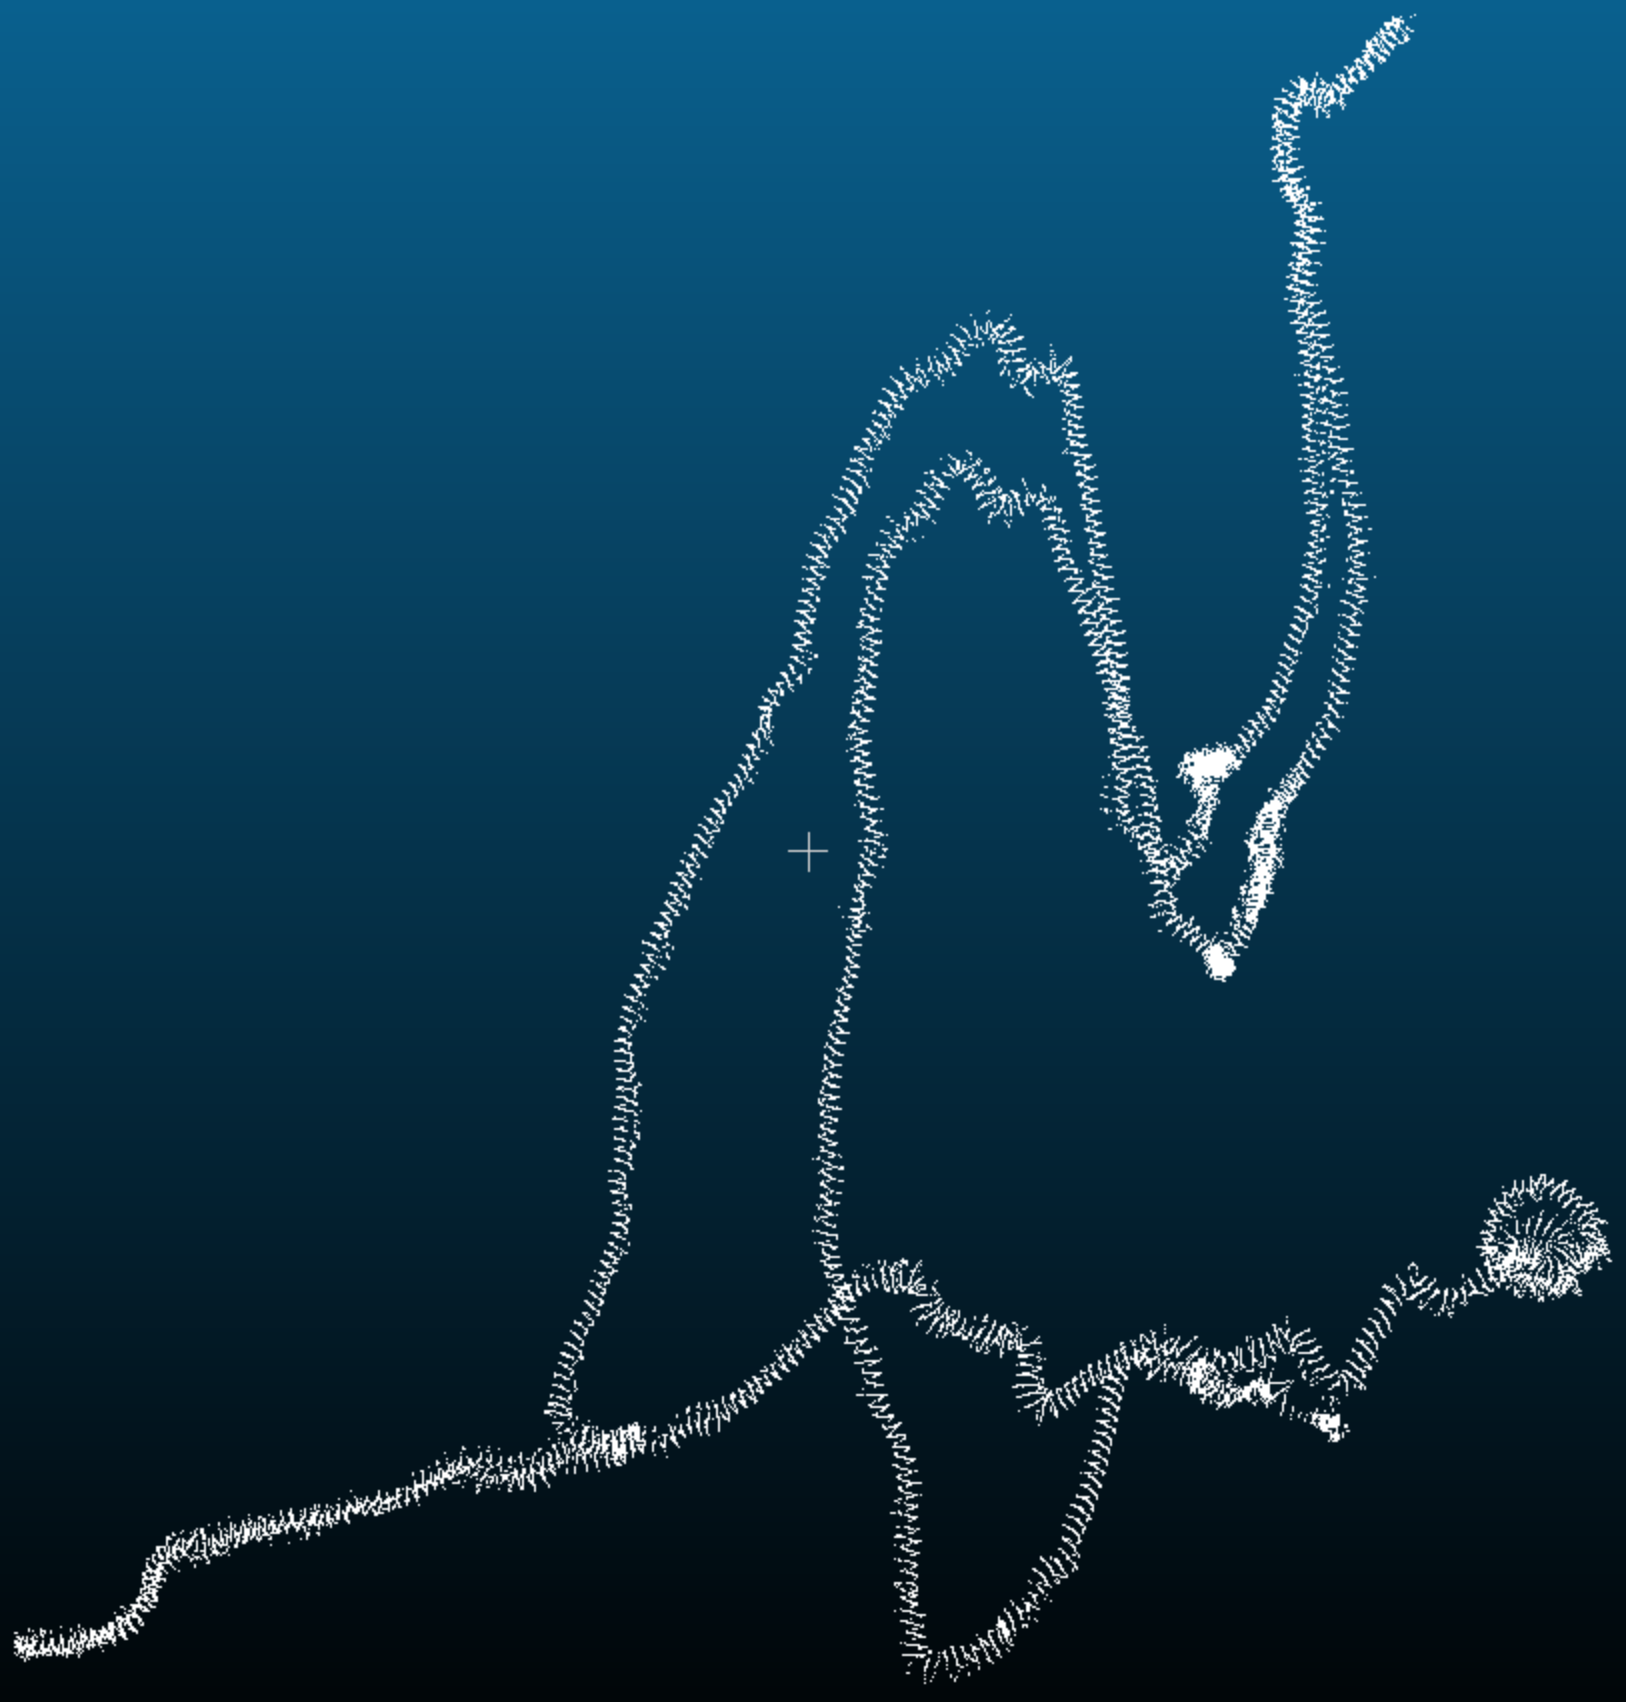
\includegraphics[width=\linewidth, height=4.5cm, keepaspectratio]{figures/RESULT_initial.png}\\[0.2em]
    {\small (a)}
  \end{minipage}\hfill
  \begin{minipage}[b]{0.32\linewidth}    % (b) horizontal sonar points
    \centering
    
\includegraphics[width=\linewidth, height=4.5cm, keepaspectratio]{figures/RESULT_horizontal.png}\\[0.2em]
    {\small (b)}
  \end{minipage}\hfill
  \begin{minipage}[b]{0.32\linewidth}    % (c) merged cloud
    \centering
    
\includegraphics[width=\linewidth, height=4.5cm, keepaspectratio]{figures/RESULT_merged.png}\\[0.2em]
    {\small (c)}
  \end{minipage}
  \caption{Point clouds of the conduit: (a) initial point cloud from the vertical sonar,
           (b) points recovered from the horizontal sonar with the estimated elevation angles,
           (c) merged point cloud.}
  \label{fig:res_merged}
\end{figure}

% ------------------------------------------------------------------------------
\subsection{Close-up comparison}         % local effect of the horizontal sonar
\label{sec:res_zoom}                     % \secref{sec:res_zoom}

At the scale of the whole conduit, the difference between the clouds is hard to judge, so
Figure~\ref{fig:res_zoom} shows a close-up of one region from the same viewpoint, without (a) and
with (b) the points of the horizontal sonar. In (a), the gaps between successive cross-sections of
the vertical sonar are visible; (b) shows how the horizontal points fill these gaps.
\hint{Comment on the local effect: how well the gaps are filled, and any region where the
horizontal points add noise.}                   % \secref{sec:res_zoom}

Figure~\ref{fig:res_zoom} compares the same region of the conduit without (a) and with (b) the
points of the horizontal sonar.
\hint{Comment on the local effect: gaps between the vertical cross-sections filled by the
horizontal points, and any region where they add noise.}

\begin{figure}[!htb]                     % zoom without / with the horizontal sonar
  \centering
  \begin{minipage}[b]{0.49\linewidth}    % (a) without the horizontal sonar
    \centering
    
\includegraphics[width=\linewidth, height=6cm, keepaspectratio]{figures/RESULT_zoom_without.png}\\[0.2em]
    {\small (a)}
  \end{minipage}\hfill
  \begin{minipage}[b]{0.49\linewidth}    % (b) with the horizontal sonar
    \centering
    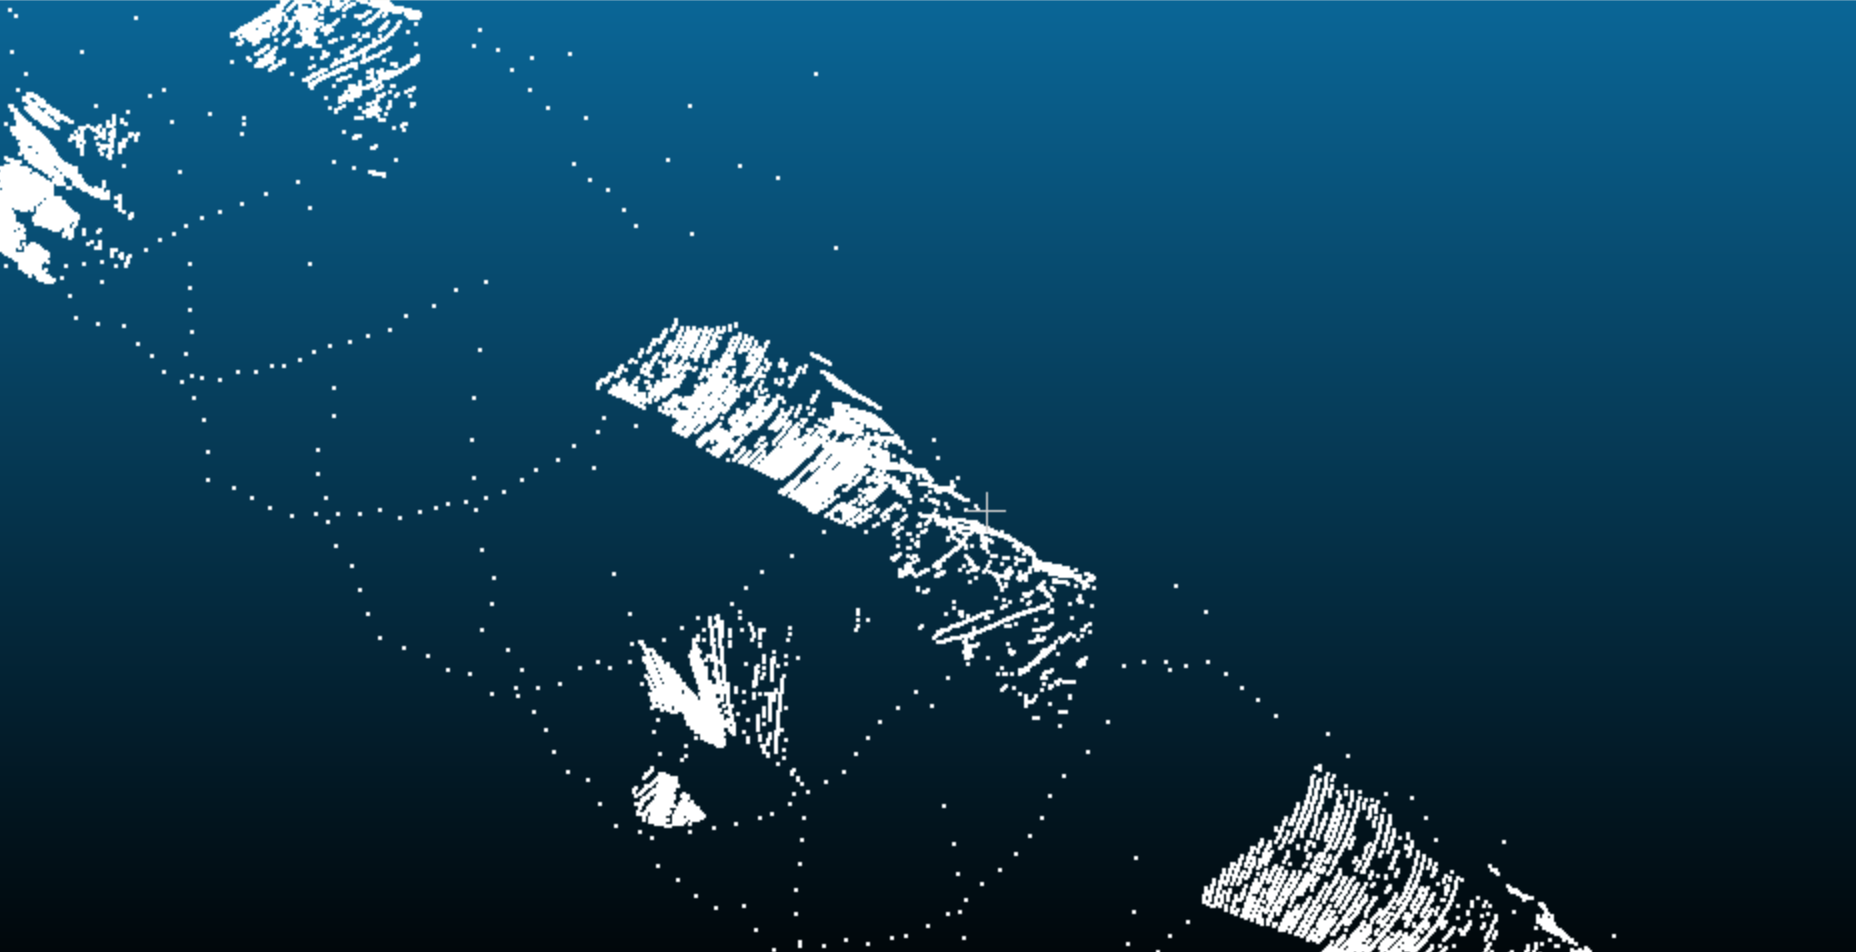
\includegraphics[width=\linewidth, height=6cm, keepaspectratio]{figures/RESULT_zoom_with.png}\\[0.2em]
    {\small (b)}
  \end{minipage}
  \caption{Close-up of the same region of the conduit, (a) without and (b) with the points of the
           horizontal sonar.}
  \label{fig:res_zoom}
\end{figure}
\section{Conclusions and Recommendations}  % obligatory
\label{sec:conclusions}                    % \secref{sec:conclusions}

\subsection{Conclusions}         % deals with the PRESENT
\hint{Summarise how the objectives stated in the introduction have been met and make
some concluding remarks.}

\subsection{Recommendations}     % deals with the FUTURE
\hint{Briefly describe the proposed plans of action for the future.}


% ---------------------------------------------------------------- end matter
\clearpage                       % appendices start on a new page
% % Confidentiality: get your employer's permission before attaching ANY company document.
\section{Appendices}             % documents supporting or clarifying the body

\subsection{Appendix A: Title of the Document}  % one subsection per appended document
\hint{Any document or information needed to support an argument or clarify something
mentioned in the body of the report. Number and title every table and figure.}

\clearpage                       % the reference list is a separate page (guide section V)
% The list is generated from references.bib: only the works you \cite appear here.
% Use \nocite{*} just above \bibliography if you want every entry printed anyway.

\bibliography{references}        % prints the section title set in setup/packages.tex


\end{document}